\documentclass[a4paper,12pt]{report}
\usepackage[english]{babel}
\usepackage{graphicx}
\usepackage{placeins}
\usepackage{hyperref}
\usepackage{supertabular}
\usepackage{tabularx}
\usepackage{listings}
\usepackage{color}
\usepackage{tipa}
\lstset{% general command to set parameter(s)
basicstyle=\footnotesize,
keywordstyle=\color{black}\bfseries\underbar,
identifierstyle=\color{black}\bfseries\underbar,
stringstyle=\ttfamily,
escapeinside={\%*}{*)},
inputencoding=utf8,
extendedchars=true,
literate={á}{{\'a}}1 {ã}{{\~a}}1 {é}{{\'e}}1 {ˈ}{{\textipa{'}}}1 {ʊ}{{\textipa{U}}}1 {ː}{{\textipa{:}}}1 {ɝ}{{\textipa{O}}}1 {æ}{{\ae}}1,
}



\parindent=0pt %no paragraph indentation
\parskip=12pt %paragraph skip
\newcommand{\HRule}{\rule{\linewidth}{0.5mm}} % Defines a new command for the horizontal lines, change thickness here

\newenvironment{devnotes}{
\begin{center}
    \begin{tabular}[h!]{|p{0.8\textwidth}|}
    \hline
    {\bf Development Notes}\\\hline}
{   \\\hline
    \end{tabular}
\end{center}}


\newcommand{\status}[2]{
\hfill {\footnotesize \textbf{Status: } {#1} $\cdot$ \textbf{Implementations: } {#2} }
}

\title{FoLiA: Format for Linguistic Annotatation}
\author{Maarten van Gompel}

\begin{document}
\sffamily

\begin{titlepage}
\begin{center}
\textsc{\large Language and Speech Technology\\ Technical Report Series}\\[1.5cm] 
\textsc{Report Number LST-14-01}\\[0.5cm] 
%\vspace{3cm}  %PRERELEASE

\HRule \\[0.5cm]
{ \Large \bfseries FoLiA: Format for Linguistic Annotation}\\[0.5cm] % Title of your document
{\bf \small version 0.11.2 -- Revision 3.9} \\[0.5cm]
{ \Large \bfseries Documentation}\\[0.5cm]
{\large \emph{Maarten van Gompel}}\\[0.5cm]
\HRule \\[1.0cm]

\emph{January 2nd, 2014 \small{(published)} -- November 26th, 2014 \small{(last revision)}} \\[0.3cm] 

\includegraphics[width=20.0mm]{ru-beeldmerk-zwart.eps}
\end{center}
\vspace{0.5cm}
%\vspace{3cm} %PRERELEASE

\begin{minipage}{0.6\textwidth}
\begin{flushleft}
PI Group Language and Speech Technology \\
Centre for Language Studies \\
Radboud University Nijmegen \\
P.O. Box 9103 \\
NL-6500 HD Nijmegen \\
The Netherlands \\
http://www.ru.nl/lst \\[0.3cm]
Series editors: \\
\hspace{0.5cm}\emph{Nelleke Oostdijk}   \\
\hspace{0.5cm}\emph{Antal van den Bosch}  \\
\hspace{0.5cm}\emph{David van Leeuwen}  \\
ISSN 2352-3107
\end{flushleft}
\end{minipage}

\end{titlepage}





\tableofcontents


\chapter{Introduction}

FoLiA is a Format for Linguistic Annotation, derived from the D-Coi
format\cite{DCOI} developed as part of the D-Coi project by project partner at
Polderland Language and Speech Technologies B.V. The D-Coi format was designed
for use by the D-Coi corpus, as well as by its successorr, the SoNaR corpus
\cite{Oostdijk+08}. Though being rooted in the D-Coi format, the FoLiA format
goes a lot further and introduces a rich generalised framework for linguistic
annotation. FoLiA development started at the ILK research group, Tilburg
University, and is continued at Radboud University Nijmegen. It is being
adopted in multiple projects in the Dutch and Flemish Natural Language
Processing community.

FoLiA is an XML-based\cite{XML} annotation format, suitable for the
representation of linguistically annotated language resources. FoLiA's intended
use is as a format for storing and/or exchanging language resources, including
corpora. Our aim is to introduce a single rich format that can accommodate a
wide variety of linguistic annotation types through a single generalised
paradigm. We do not commit to any label set, language or linguistic theory.
This is always left to the developer of the language resource, and provides
maximum flexibility.

XML is an inherently hierarchic format. FoLiA does justice to this by maximally
utilising a hierarchic, inline, setup. We inherit from the D-Coi format, which
posits to be loosely based on a minimal subset of TEI\cite{TEI}. Because of the
introduction of a new and much broader paradigm, FoLiA is \emph{not}
backwards-compatible with D-Coi, i.e. validators for D-Coi will not accept
FoLiA XML. It is, however, easy to convert FoLiA to less complex or verbose
formats such as the D-Coi format, or plain-text. Converters will be provided.
This may entail some loss of information if the simpler format has no
provisions for particular types of information specified in the FoLiA format. 

The most important characteristics of FoLiA are:

\begin{itemize}
\item \textbf{Generalised} paradigm - We use a generalised paradigm, with as few ad-hoc provisions for annotation types as possible.
\item \textbf{Expressivity} - The format is highly expressive, annotations can be expressed in great detail and with flexibility to the user's needs, without forcing unwanted details. Moreover, FoLiA has generalised support for representing annotation alternatives, and annotation metadata such as information on annotator, time of annotation, and annotation confidence.
\item \textbf{Extensible} - Due to the generalised paradigm and the fact that the format does not commit to any label set, FoLiA is fairly easily extensible.   
\item \textbf{Formalised} - The format is formalised, and can be validated on both a shallow and a deep level (the latter including tagset validation), and easily machine parsable, for which tools are provided.
\item \textbf{Practical} - FoLiA has been developed in a bottom-up fashion right alongside applications, libraries, and other toolkits and converters. Whilst the format is rich, we try to maintain it as simple and straightforward as possible, minimising the learning curve and making it easy to adopt FoLiA in practical applications.  
\end{itemize}

The FoLiA format makes mixed-use of inline and stand-off annotation. Inline annotation is used for annotations pertaining to single tokens, whilst stand-off annotation in a separate annotation layers is adopted for annotation types that span over multiple tokens. This provides FoLiA with the necessary flexibility and extensibility to deal with various kinds of annotations. Inspiration for this was in part obtained from the Kyoto Annotation Format \cite{KYOTO}.

In publication of research that makes use of FoLiA, a citation should be given
of: {\em ``Maarten van Gompel (2013). FoLiA: Format for Linguistic Annotation.
Documentation. Language and Speech Technology Technical Report Series 13-01.
Radboud University Nijmegen.''}. The latest version of the documentation is
always available from {\tt http://proycon.github.io/folia}.  FoLiA is
open-source and all technical resources are licensed under the GNU Public
License v3.

\medskip
Notable features of the FoLiA format include:

\begin{itemize}
\item XML-based, validation against RelaxNG schema.
\item Full Unicode support; UTF-8 encoded.
\item Support for text as well as speech
\item Document structure consists of divisions, paragraphs, sentences and words/tokens, and more specific elements.
\item Support for annotation of transcribed speech
\item Can be used for both tokenised as well as untokenised text, though for meaningful linguistic annotation, tokenisation is mandatory.
\item Provenance support for all linguistic annotations: annotator, type (automatic or manual), time.
\item Support for alternative annotations, optionally with associated confidence values.
\item Support for features using subsets, allowing for more detailed user-defined annotation.
\item Not commited to any label set, label sets are user-defined.
\item Agnostic with regard to metadata. External metadata schemes such as CMDI
  \cite{CMDI} are recommended.
\end{itemize}

There is support for the following linguistic annotations:

\begin{itemize}
\item Part-of-speech tags (with features)
\item Lemmatisation
\item Spelling corrections on both a tokenised as well as an untokenised level
\item Lexical semantic sense annotation 
\item Named Entities / Multi-word units
\item Syntactic Parses
\item Dependency Relations
\item Chunking
\item Morphological Analysis
\item Subjectivity Annotation/Sentiment analysis
\item Semantic Role Labelling
\item Co-reference
\item Event annotation
\end{itemize}

FoLiA support is incorporated directly into the following software:

\begin{itemize} 
\item ucto - A tokeniser which can directly output FoLiA XML 
\item Frog - A PoS-tagger/lemmatiser/parser suite (the successor of Tadpole), will eventually support reading and writing FoLIA.
\item CLAM - Computational Linguistics Application Mediator, will eventually have viewers for the FoLiA format.
\item PyNLPl - Python Natural Language Processing Library, comes with a library for parsing FoLiA
\item libfolia - C++ library for parsing FoLiA
\end{itemize}

FoLiA is used in various projects (list may not be complete):

\begin{itemize}
\item SoNaR (STEVIN)
\item DutchSemCor (NWO)
\item TTNWW (CLARIN)
\item DU-VNC (CLARIN)
\item Ticclops (CLARIN)
\item Valkuil.net
\item Basilex (NWO)
\item LIN (NWO)
\end{itemize}

To clearly understand this documentation, note that when we speak of ``elements'' or ``attributes'', we refer to XML notation, i.e. XML elements and XML attributes.

\section{Status Information}

The FoLiA format, this documentation, and the libraries implementing FoLiA are a constant work in progress. In this documentation, the status and implementation of a certain annotation type is indicated as follows:

\status{final since v0.4}{pynlpl,libfolia}

The above example states that the particular section is final since version 0.4 of FoLiA and that it is implemented in the libraries pynlpl (python) and libfolia ($C++$). You may also see portions of this documentation that are proposals, which means the functionality is still open for debate and not final yet. Example: 

\status{PROPOSED in v0.9)}{not implemented yet} 

Any version of FoLiA and its libraries should be compatible with earlier releases. When things have changed between versions, this is indicated in the documentation. 

\chapter{Document Format}

\section{Global Structure}

In FoLiA, each document/text is represented by one XML file. The basic structure of such a FoLiA document is as follows and should always be UTF-8 encoded.

\begin{lstlisting}[language=xml]
<?xml version="1.0" encoding="utf-8"?>
<FoLiA xmlns="http://ilk.uvt.nl/FoLiA"
  xmlns:xsi="http://www.w3.org/2001/XMLSchema-instance" 
  version="0.5"
  xml:id="example">
  <metadata>
      <annotations>
          ...
      </annotations> 
  </metadata>
  <text xml:id="example.text">
     ...
  </text>
</FoLiA>  
\end{lstlisting}



\section{Identifiers}

Many elements in the FoLiA format specify an identifier by which the element is uniquely identifiable. This makes referring to any part of a FoLiA document easy and follows the lead of the D-Coi format. Identifiers should be unique in the entire document, and can be anything that qualifies as a valid ID according to the XML standard. A well proven convention is of a cumulative nature, in which you append the element name, a period, and a sequence number, to the identifier of a parent element higher in the hierarchy. Identifiers are always encoded in the \texttt{xml:id} attribute.

The FoLiA document as a whole also carries an ID.

Identifiers are very important and used throughout the FoLiA format, and mandatory for almost all structural elements. They enable external resources and databases to easily point to a specific part of the document or an annotation therein. FoLiA has been set up in such a way that \emph{identifiers should never change}. Once an identifier is assigned, it should never change, re-numbering is strictly prohibited unless you intentionally want to create a new resource and break compatibility with the old one.

 
\section{Paradigm \& Terminology}
\label{sec:paradigm}

The FoLiA format has a very uniform setup and its XML notation for annotation follows a generalised paradigm. We distinguish several different categories of annotation, three main categories and several higher-order annotation categories.

\begin{itemize}
\item \textbf{Structural annotation} - Annotations marking global structure, such as chapters, sections, subsections, figures, list items, paragraphs, sentences, words, morphemes, phonemes etc... Section~\ref{sec:structureannotation} will discuss most structure annotation elements in FoLiA. Morphemes and phonemes are discusses in separate sections. 
\item \textbf{Token annotation} - Annotations pertaining to a specific token. These will be elements of the token element (\texttt{w}) in inline notation. Linguistic annotations in this category are for example: part-of-speech annotation (lexical categories), lemma annotation, sense annotation. Various token annotation elements may be used on higher levels (e.g. sentence/paragraph) as well and may then be referred to as \textbf{Extended Token Annotation}. Section~\ref{sec:tokenannotation} will discuss all token annotations.
\item \textbf{Span annotation} - Annotations spanning over multiple tokens.
  Each type of annotation will be in a separate \textbf{annotation layer} with
  stand-off notation. These layers are typically embedded on the sentence
  level, or possibly also on higher levels (paragraph/division/text) for
  certain annotation types. Examples in this category are: the labelling of
  syntactic constituent structure, syntactic dependencies, chunks, co-reference, semantic roles and named entities. Section~\ref{sec:spanannotation} will discuss all span annotations.
\item \textbf{Higher-order annotation} - Higher-order annotation consists of several categories of annotation. These all have in common that they annotate either other annotations, or in some way modify or point at other annotations. 
\begin{itemize}
	\item \textbf{Feature annotation} - Feature annotation allows for more detailed annotation. It acts as a feature or attribute to an annotation. This category of annotation will be explained in Section~\ref{sec:features}.
	\item \textbf{Alignment annotation} - Allows for associations between arbitrary annotations within or across FoLiA documents.
	\item \textbf{Corrections} - Allows corrections or suggestions for correction to be associated with annotations.
	\item \textbf{Alternatives} - Allows annotations to be marked as alternative.
\end{itemize}

%\item \textbf{Subtoken annotation} - This is a type of annotation that has aspects of both token annotation as well as span annotation. The former because it is included inline within a token element (\texttt{w}) and describes the token. The latter because is defines a small span \emph{within} the token. Examples in this category are: morphological analysis. %TODO %DEPRECATED
\end{itemize}

Almost all annotations are associated with what we call a \textbf{set}. The set
determines the vocabulary of the annotation, i.e. the tags or types of the
annotation. An element of such a set is referred to as a \textbf{class}. For
example, we may have a document with Part-of-speech annotation according to the
CGN set, a tagset for Dutch part-of-speech tags \cite{CGN}. The CGN set defines
main tag classes such as \emph{WW}, \emph{BW}, \emph{ADJ}, \emph{VZ}. FoLiA
itself thus never commits to any tagset but leaves you to define this. You can
also use multiple tagsets in the same document if so desired, even for the same
type of annotation.

Any annotation element may have a \texttt{set} attribute, the value of which points to the URL of the set definition file that defines the set. Such an element then also carries a \texttt{class} attribute, which selects a particular class from the set.

In addition to this, various other generic FoLiA attributes are available for all annotation elements. These are never mandatory:

\begin{enumerate}
\item \texttt{annotator} -- The name or ID of the system or human annotator that made the annotation.
\item \texttt{annotatortype} -- ``manual'' for human annotators, or ``auto'' for automated systems.
\item \texttt{confidence} -- A floating point value between zero and one; expresses the confidence the annotator places in his annotation.
\item \texttt{datetime} --  The date and time when this annotation was recorded, the format is \texttt{YYYY-MM-DDThh:mm:ss} (note the T in the middle to separate date from time), as per the XSD Datetime data type.
\item \texttt{n} --  A number in a sequence, corresponding to a number in the original document, for example chapter numbers, section numbers, list item numbers.
\end{enumerate}

The following example shows a simple Part-of-speech annotation without features, but with various generic attributes according:

\begin{lstlisting}[language=xml]
<pos set="http://ilk.uvt.nl/folia/sets/CGN" class="WW" 
 annotator="Maarten van Gompel" annotatortype="manual"
 confidence="0.76" datetime="1982-12-15T19:01" />
\end{lstlisting}

The FoLiA paradigm is visualised in Figure~\ref{fig:paradigm}. Note that the more advanced aspects of the FoLiA paradigm, the higher-order annotation categories, will be introduced later in Section~\ref{sec:higherorder}.

\begin{figure}[h]
\begin{center}
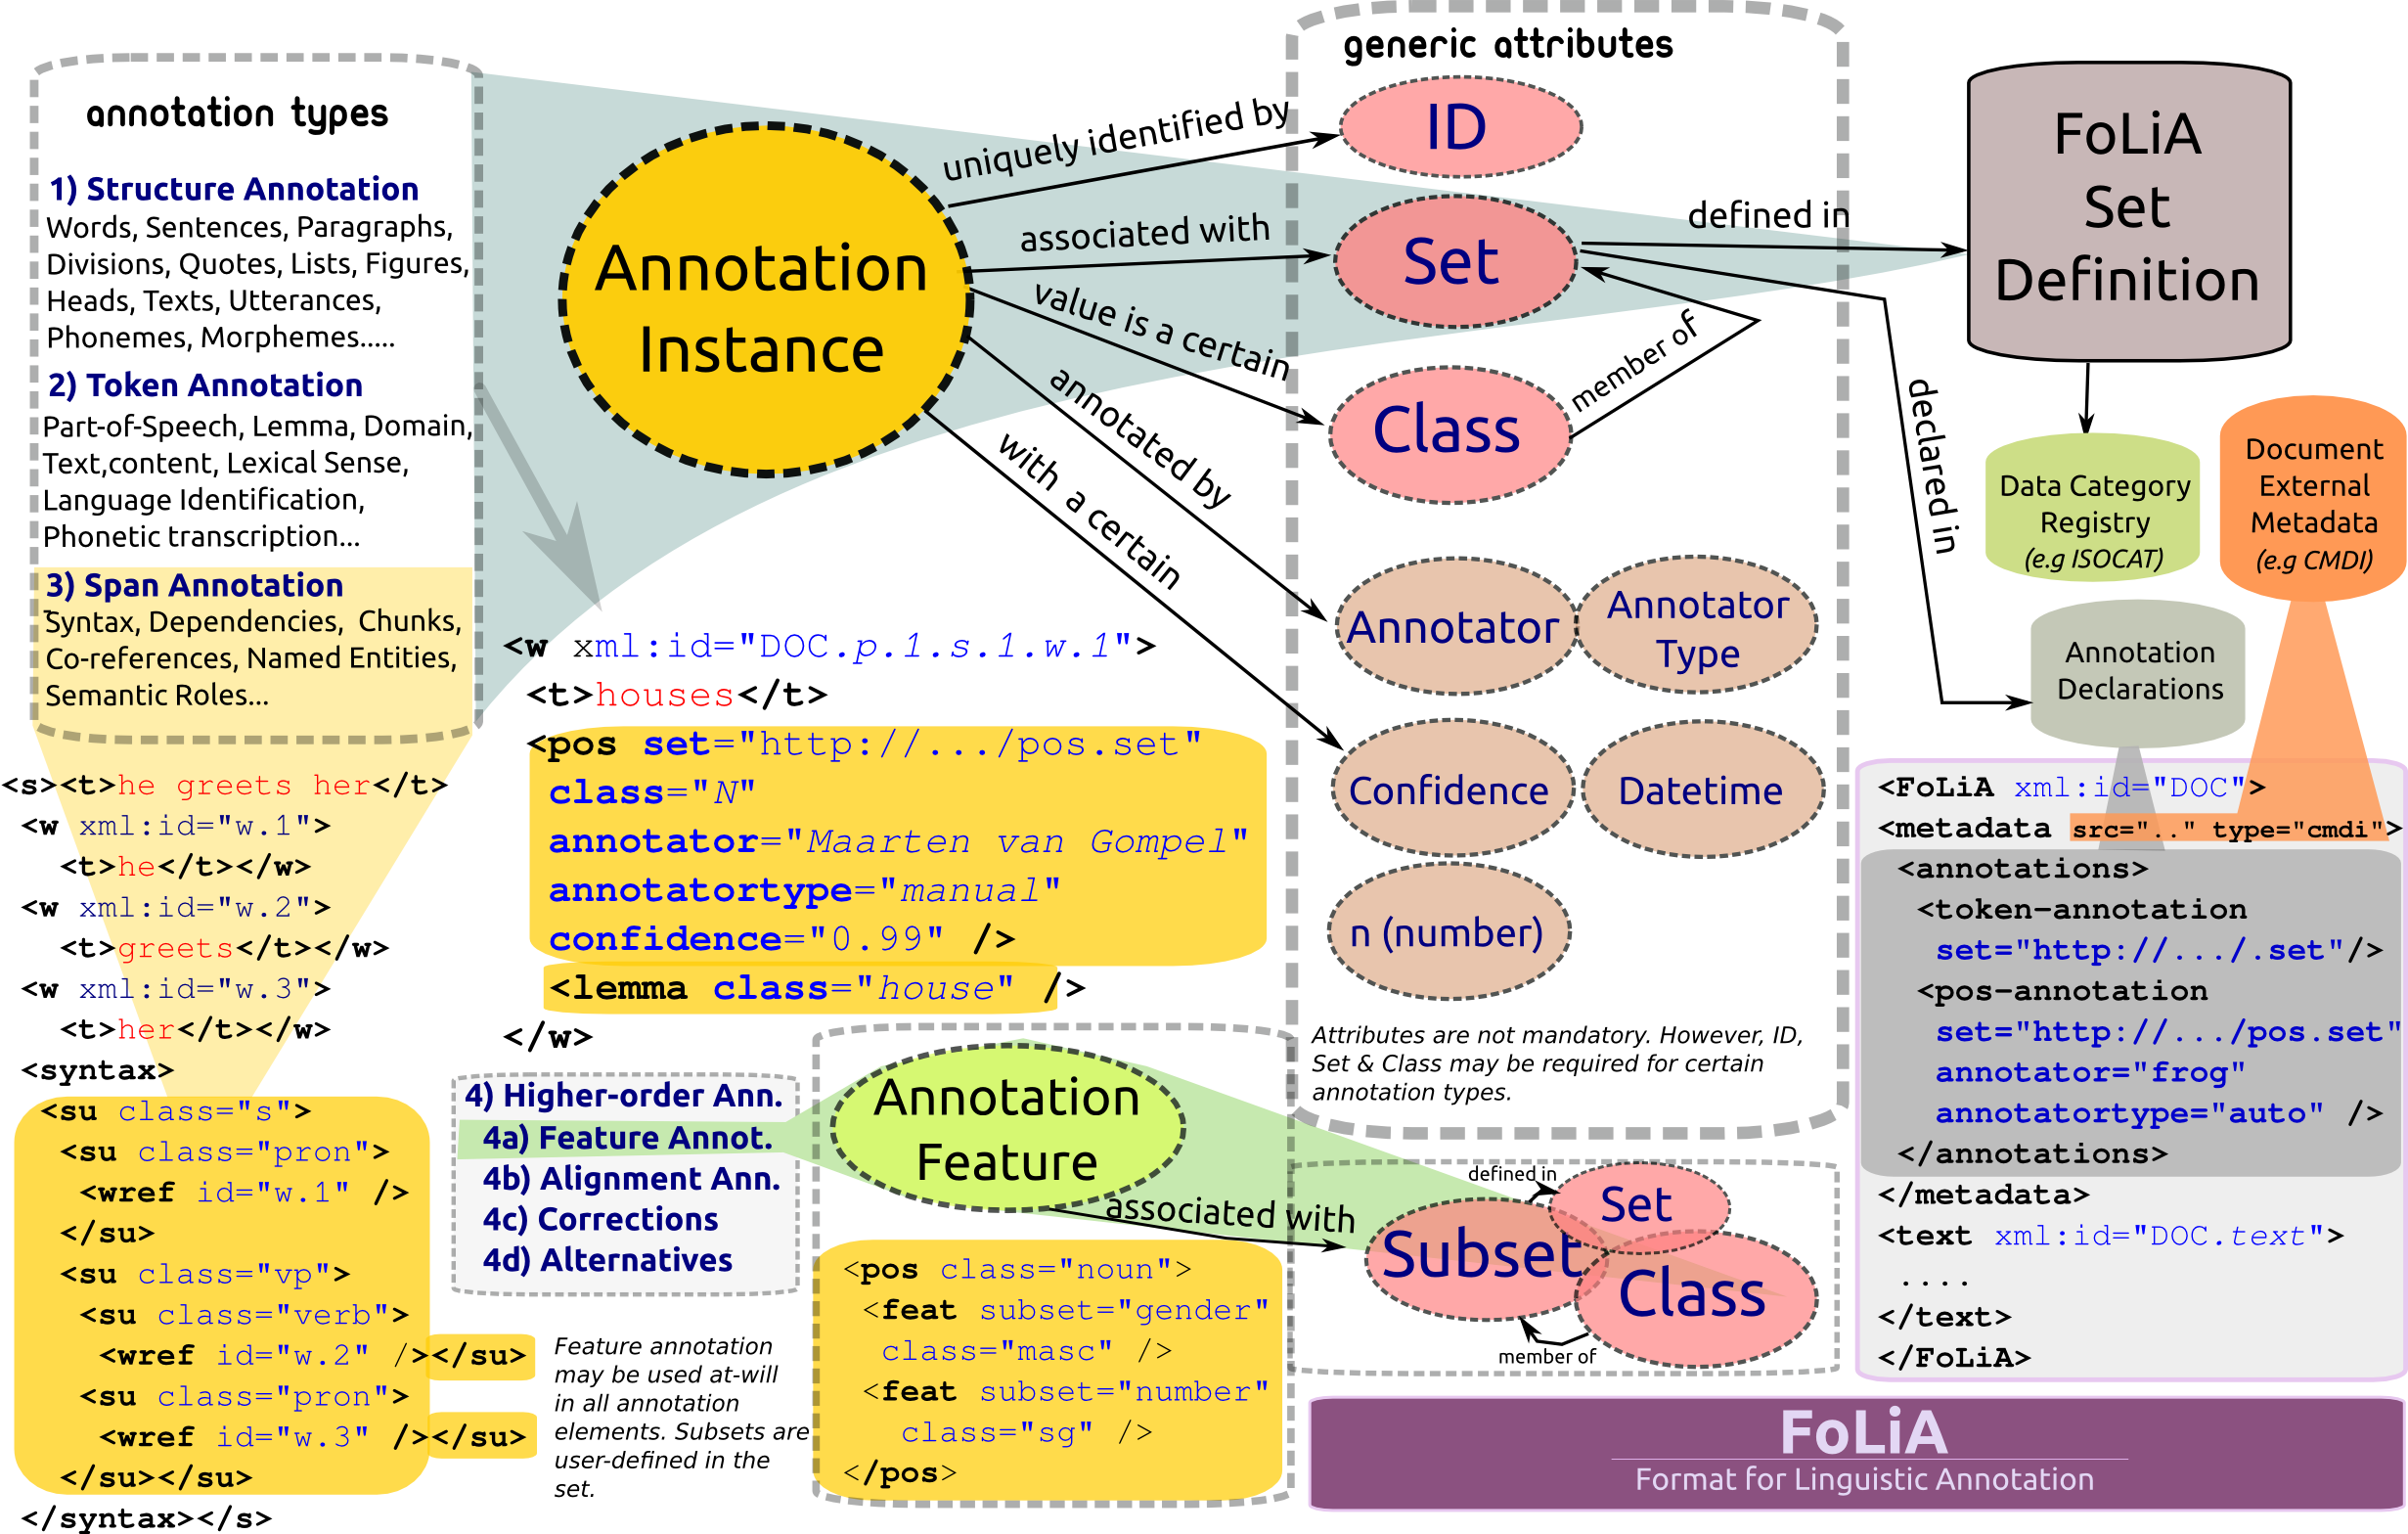
\includegraphics[width=145.0mm]{folia_paradigm.png}
\end{center}
\caption{The FoLiA Paradigm}
\label{fig:paradigm} 
\end{figure}

\subsection{Speech}
\label{sec:speechparadigm}

\status{PROPOSED in v0.9)}{not implemented yet}

FoLiA is also suited for annotation of speech data. The following additional FoLiA attributes are available for \emph{all} structure annotation elements in a speech context: 

\begin{itemize}
  \item \texttt{src} -- \textbf{source} -- Points to a file or full URL of a sound or video file. This attribute is inheritable.
   
  \item \texttt{begintime} -- \textbf{begin time} --  A timestamp in
    \texttt{HH:MM:SS.MMMM} format, indicating the begin time of the speech. If a sound clip is specified (\texttt{src}); the timestamp refers to a location in the soundclip (minus \texttt{srcoffset}).
    
  \item \texttt{endtime} -- \textbf{end time} --  A timestamp in
    \texttt{HH:MM:SS.MMMM} format, indicating the end time of the speech. If a sound clip is specified (\texttt{src}); the timestamp refers to a location in the soundclip (minus \texttt{srcoffset}).
  
  \item \texttt{srcoffset} -- \textbf{source offset} -- A timestamp in \texttt{HH:MM:SS.MMMM} format that is \emph{subtracted} from all \texttt{begintime}, and \texttt{endtime} designations within its scope, to find the position in the audio clip. This attribute enables the use of global timings in all begintime/endtime attributes, across different sound clips. Defaults to zero.
  
  \item \texttt{speaker} -- \textbf{speaker} -- A string identifying the
    speaker. This attribute is inheritable. Multiple speakers are not allowed,
    simply do not specify a speaker on a certain level if you are unable to
    link the speech to a specific (single) speaker.
\end{itemize}
 
More about speech annotation in Section~\ref{sec:speech}.

\section{Annotation Declaration}
\label{sec:declarations}

The annotation declaration is a mandatory part of the metadata that declares all types of annotation and all sets that are present in the document. Annotations are declared in the \texttt{annotations} block, as shown in the following example. We here define four annotation levels with fictitious sets:

\begin{lstlisting}[language=xml]
<annotations>
        <token-annotation 
          set="http://ilk.uvt.nl/folia/sets/ucto-tokconfig-nl" 
          annotator="ucto" annotatortype="auto" />
        <pos-annotation set="http://ilk.uvt.nl/folia/sets/CGN" 
          annotator="Frog" annotatortype="auto" />
        <lemma-annotation set="http://ilk.uvt.nl/folia/sets/lemmas-nl" 
          annotator="Frog" annotatortype="auto" />    
        <sense-annotation set="http://ilk.uvt.nl/folia/sets/Cornetto"
         annotator="SupWSD1" annotatortype="auto" />    
</annotations>
\end{lstlisting}

The set attribute is mandatory\footnote{Technically, it can be omitted, but
then the set defaults to ``undefined''. This is allowed for flexibility and
less explicit usage of FoLiA in limited settings, but not recommended!} and
refers to a URL of a FoLiA Set Definition file (see
Chapter~\ref{chapter:setdefinitions}). In the above example, the set URLs are
fictitious, make sure to list your own appropriate sets. A Set Definition
specifies exactly what classes are allowed in the set. It for examples
specifies exactly what Part-of-speech tags exist. This information is necessary
to x validate the document completely at its deepest level. If the sets point
to URLs that do not exist or are not URLs at all, warnings will be issued.
Validation can still proceed but with the notable exception of deep validation
of these sets.

If multiple sets are used for the same annotation type, they each need a separate declaration:

\begin{lstlisting}[language=xml]
        <pos-annotation set="http://ilk.uvt.nl/folia/sets/CGN" 
          annotator="Frog" annotatortype="auto" />
        <pos-annotation set="http://ilk.uvt.nl/folia/sets/brown" />
\end{lstlisting}

If only one set is declared, then in the document itself you are allowed to skip the set attribute on these specific annotation elements. The declared set will automatically be the default. 

The \texttt{annotator} and \texttt{annotatortype} attributes act as defaults for the specific annotation type and set. Unlike \texttt{set}, you do \emph{not} need, and it is in fact prohibited, to declare every possible annotator here!

Annotator defaults can always be overridden at the specific annotation elements. But declaring them allows for the annotation element to be less verbosely expressed. Explicitly referring to a set and annotator for each annotation element can be cumbersome and pointless in a document with a single set and a single annotator for that particular type of annotation. Declarations and defaults provide a nice way around this problem.


\section{Structure Annotation}
\label{sec:structureannotation}

\subsection{Basic Structural Elements}
\label{sec:basics}

Basic structural elements for textual documents occur within the \texttt{text} element. These are the most basic ones:

\begin{itemize}
\item \texttt{p} - Paragraph
\item \texttt{s} - Sentence
\item \texttt{w} - Word (token)
\end{itemize}

These are typically nested, the word elements cover the actual tokens. This is
the most basic level of annotation; tokenisation. Let's take a look at an
example where we have the following text:

\begin{verbatim}
This is a paragraph containing only one sentence.

This is the second paragraph. This one has two sentences.
\end{verbatim}

In FoLiA XML, this will appear as follows after tokenisation. Some parts have been omitted for the sake of brevity:

\begin{lstlisting}[language=xml]
 <p xml:id="example.p.1">
    <s xml:id="example.p.1.s.1">        
        <w xml:id="example.p.1.s.1.w.1"><t>This</t></w>
        <w xml:id="example.p.1.s.1.w.2"><t>is</t></w>
        ...
        <w xml:id="example.p.1.s.1.w.8" space="no"><t>sentence</t></w>
        <w xml:id="example.p.1.s.1.w.9"><t>.</t></w>
    </s>
 </p>
 <p xml:id="example.p.2">
    <s xml:id="example.p.2.s.1">
        <w xml:id="example.p.2.s.1.w.1"><t>This</t></w>
        <w xml:id="example.p.2.s.1.w.2"><t>is</t></w>    
        ..
        <w xml:id="example.p.2.s.1.w.5" space="no"><t>paragraph</t></w>    
        <w xml:id="example.p.2.s.1.w.6"><t>.</t></w>    
    </s>
    <s xml:id="example.p.2.s.2">
        <w xml:id="example.p.2.s.2.w.1"><t>This</t></w>
        <w xml:id="example.p.2.s.2.w.2"><t>one</t></w>    
        ..
        <w xml:id="example.p.2.s.2.w.5" space="no"><t>sentences</t></w>    
        <w xml:id="example.p.2.s.2.w.6"><t>.</t></w>    
    </s>
 </p>
\end{lstlisting}

FoLiA is not just a format for holding tokenised text, although tokenisation is a prerequisite for almost all kinds of annotation. However, FoLiA can also hold untokenised text, on for example paragraph and/or sentence level:

\begin{lstlisting}[language=xml]
 <p xml:id="example.p.1">
    <s xml:id="example.p.1.s.1">        
        <t>This is a paragraph containing only one sentence.</t>
    </s>
 </p>
 <p xml:id="example.p.2">
    <s xml:id="example.p.2.s.1">     
        <t>This is the second paragraph.</t>
    </s>
    <s xml:id="example.p.2.s.2">     
        <t>This one has two sentences.</t>
    </s>    
 </p>
\end{lstlisting}

Higher level elements \emph{may} also contain a text element even when the deeper elements do too. It is very important to realise that the sentence/paragraph-level text element \emph{always} contains the text \emph{prior} to tokenisation! Note also that the word element has an attribute \texttt{space}, which defaults to yes, and indicates whether the word was followed by a space in the \emph{untokenised} original. This allows for partial reconstructibility of the sentence in its untokenised form. See Section~\ref{sec:textcontent} for a more elaborate overview of this subject.

The following example shows the maximum amount of redundancy, with text elements at every level.

\begin{lstlisting}[language=xml]
 <p xml:id="example.p.1">
    <t>This is a paragraph containing only one sentence.</t>
    <s xml:id="example.p.1.s.1">        
        <t>This is a paragraph containing only one sentence.</t>
        <w xml:id="example.p.1.s.1.w.1"><t>This</t></w>
        <w xml:id="example.p.1.s.1.w.2"><t>is</t></w>
        ...
        <w xml:id="example.sp.1.s.1.w.8" space="no"><t>sentence</t></w>
        <w xml:id="example.p.1.s.1.w.9"><t>.</t></w>
    </s>
 </p>
 <p xml:id="example.p.2">
    <t>This is the second paragraph. This one has two sentences.</t>
    <s xml:id="example.p.2.s.1">
        <t>This is the second paragraph.</t>
        <w xml:id="example.p.2.s.1.w.1"><t>This</t></w>
        <w xml:id="example.p.2.s.1.w.2"><t>is</t></w>    
        ..
        <w xml:id="example.p.2.s.1.w.5" space="no"><t>paragraph</t></w>    
        <w xml:id="example.p.2.s.1.w.6"><t>.</t></w>    
    </s>
    <s xml:id="example.p.2.s.2">
        <t>This one has two sentences.</t>
        <w xml:id="example.p.2.s.2.w.1"><t>This</t></w>
        <w xml:id="example.p.2.s.2.w.2"><t>one</t></w>    
        ..
        <w xml:id="example.p.2.s.2.w.5" space="no"><t>sentences</t></w>    
        <w xml:id="example.p.2.s.2.w.6"><t>.</t></w>    
    </s>
 </p>
\end{lstlisting}

If this kind of redundancy is used (it is not mandatory), you may optionally point back to the text content of its parent by specifying the \texttt{offset} attribute:

\begin{lstlisting}[language=xml]
 <p xml:id="example.p.1">
    <t>This is a paragraph containing only one sentence.</t>
    <s xml:id="example.p.1.s.1">        
        <t offset="0">This is a paragraph containing only one sentence.</t>
        <w xml:id="example.p.1.s.1.w.1">
        	<t offset="0">This</t>
        </w>
        <w xml:id="example.p.1.s.1.w.2">
        	<t offset="5">is</t>
        </w>
        ...
        <w xml:id="example.p.1.s.1.w.8" space="no">
        	<t offset="40">sentence</t>
        </w>
        <w xml:id="example.p.1.s.1.w.9">
        	<t offset="48">.</t>
        </w>
    </s>
 </p>
\end{lstlisting}

Matters can become more complicated as multiple text-content element of
different classes may be associated with an element, this will be discussed
later on in Section~\ref{sec:textcontent}.

Paragraph elements may be omitted if a document is described that does not
distinguish paragraphs but only sentences. Sentences, however, may never be
omitted; FoLiA documents can never consist of tokens only.

The content element \texttt{head} is reserved for headers and captions, it
behaves similarly to the paragraph element and holds sentences.

FoLiA also explicitly supports quotes, as demonstrated in the next example, which annotates the following sentence: 

\begin{verbatim}
He said: ``I do not know . I think you are right. ", and left.
\end{verbatim}

A quote may consist of one or more sentences, but may also consist of mere tokens:

\begin{lstlisting}[language=xml]
 <s xml:id="example.p.1.s.1">
  <w xml:id="example.p.1.s.1.w.1" class="WORD"><t>He</t></w>
  <w xml:id="example.p.1.s.1.w.2" class="WORD"><t>said</t></w>
  <w xml:id="example.p.1.s.1.w.3" class="PUNCTUATION" space="no">
  	<t>:</t>
  </w>
  <w xml:id="example.p.1.s.1.w.4" class="PUNCTUATION" space="no">
  	<t>''</t>
  </w>
  <quote xml:id="example.p.1.s.1.quote.1">
    <s xml:id="example.p.1.s.1.quote.1.s.1">
       <w xml:id="example.p.1.s.1.w.5" class="WORD"><t>I</t></w>
       <w xml:id="example.p.1.s.1.w.6" class="WORD"><t>do</t></w>
       <w xml:id="example.p.1.s.1.w.7" class="WORD"><t>not</t></w>
       <w xml:id="example.p.1.s.1.w.8" class="WORD"><t>know</t></w>
       <w xml:id="example.p.1.s.1.w.9" class="PUNCTUATION" space="no">
       	<t>.</t>
       </w>
    </s>
    <s xml:id="example.p.1.s.1.quote.1.s.2">
       <w xml:id="example.p.1.s.1.w.10" class="WORD"><t>I</t></w>
       <w xml:id="example.p.1.s.1.w.11" class="WORD"><t>think</t></w>
       <w xml:id="example.p.1.s.1.w.12" class="WORD"><t>you</t></w>
       <w xml:id="example.p.1.s.1.w.13" class="WORD"><t>are</t></w>
       <w xml:id="example.p.1.s.1.w.14" class="WORD"><t>right</t></w>
    </s>
  </quote>
  <w xml:id="example.p.1.s.1.w.15" class="PUNCTUATION" space="no">
   <t>''</t>
  </w>
  <w xml:id="example.p.1.s.1.w.16" class="PUNCTUATION"><t>,</t></w>
  <w xml:id="example.p.1.s.1.w.17" class="WORD"><t>and</t></w>
  <w xml:id="example.p.1.s.1.w.18" class="WORD"><t>left</t></w>
  <w xml:id="example.p.1.s.1.w.19" class="PUNCTUATION" space="no">
  	<t>.</t>
  </w>
 </s>
\end{lstlisting}


\subsection{Paragraphs, Sentences and Words}

Paragraphs, sentences and words (or tokens) are amongst the most elementary
structure elements. As we saw in a previous section, word elements (\texttt{w})
can take a class, pertaining to a certain set, at which point a definition must
be present in the metadata, note that the actual set URL is just an example.
You should assign your own:

\begin{lstlisting}[language=xml]
<annotations>
    <token-annotation set="http://ilk.uvt.nl/folia/sets/ucto-tokconfig-nl"
      annotator="ucto" annotatortype="auto" />
</annotations>
\end{lstlisting}

Being part of a set, this implies that tokens themselves \emph{may} be assigned a class, as is for example done by the tokeniser \emph{ucto}:

\begin{lstlisting}[language=xml]
<s xml:id="example.p.1.s.1">
	<t>I see 2 children.</t>
    <w xml:id="example.p.1.s.1.w.1" class="WORD"><t>I</t></w>
    <w xml:id="example.p.1.s.1.w.2" class="WORD"><t>see</t></w>
    <w xml:id="example.p.1.s.1.w.3" class="NUMBER"><t>2</t></w>
    <w xml:id="example.p.1.s.1.w.4" class="WORD" space="no">
		<t>children</t>
    </w>
    <w xml:id="example.p.1.s.1.w.5" class="PUNCTUATION"><t>.</t></w>
</s>
\end{lstlisting}        

The same can be applied to paragraphs and sentences, which requires a declaration of \texttt{paragraph-annotation} and \texttt{sentence-annotation} respectively.

\subsection{Divisions}

Within the \texttt{text} element, the structure element \texttt{div} can be used to create divisions and subdivisions. Each division \emph{may} be of a particular \emph{class} pertaining to a \emph{set} defining all possible classes.

Divisions and other structural units are often numbered, think for example of chapters and sections. The number, as it was in the source document, can be encoded in the \texttt{n} attribute of the structure annotation element.

Look at the following example, showing a full FoLiA document with structured divisions. The declared set is a fictitious example:

\begin{lstlisting}[language=xml]
<?xml version="1.0" encoding="utf-8"?>
<?xml-stylesheet type="text/xsl" 
 href="http://ilk.uvt.nl/FoLiA/FoLiA.xsl"?>
<FoLiA xmlns="http://ilk.uvt.nl/FoLiA"
  xmlns:xsi="http://www.w3.org/2001/XMLSchema-instance" 
  version="0.5"
  xml:id="example">
  <metadata>
      <annotations>
          <division-annotation 
           set="http://ilk.uvt.nl/folia/sets/divisions" />
      </annotations>    
  </metadata>
  <text xml:id="example.text">
     <div class="chapter" n="1">
        <head><t>Introduction</t></head>
        <div class="section" n="1">
            <div class="subsection" n="1.1">
                <t>In the beginning....</t>
            </div>
        </div>
        ...
     </div>
  </text>
</FoLiA>  
\end{lstlisting}

Divisions stem from D-Coi and are modified in FoLiA. These divisions are not
mandatory, but may be used to mark extra structure. D-Coi supports the elements
\texttt{div0}, \texttt{div1}, \texttt{div2}, etc.., but FoLiA only knows a
single \texttt{div} element, which can be nested at will and associated with
classes. Note that paragraphs, sentences and words have there own explicit
tags, as we saw earlier, divisions should never be used for marking these, only larger structures can be divisions.

The \texttt{head} element may be used for the header of any division. It may hold \texttt{s} and \texttt{w} elements (not \texttt{p}).


\subsection{Gaps}

\status{final since v0.8 (older versions are equal but lack declarations)}{pynlpl, libfolia}

Sometimes there are parts of a document you want to skip and not annotate, but include as is. For this purpose the \texttt{gap} element should be used. Gaps may have a particular class indicating the kind of gap it is. Common omissions are for example front-matter and back-matter.

The D-Coi format pre-defines the following ``reasons'' \cite{DCOI}:

\begin{itemize}
\item frontmatter
\item backmatter
\item illegible
\item other-language
\item cancelled
\item inaudible
\item sampling
\end{itemize}

Due to the flexible nature of FoLiA, we never predefine any classes whatsoever and leave this up to whatever set is declared. The above gives a good indication of what gaps can be used for though. 

The gap element may optionally take two elements:

\begin{enumerate}
\item \texttt{desc} - holding a substitute that may be shown to the user, describing what has been omitted.
\item \texttt{content} - The actual raw content of the omission, as it was without further annotations. This is an XML CDATA type element, excluding it from any kind of parsing.
\end{enumerate}


\begin{lstlisting}[language=xml]
  <text xml:id="example.text">
     <gap class="frontmatter" annotator="Maarten van Gompel">
        <desc>This is the cover of the book</desc>
        <content>
<![CDATA[        
    
            SHOW WHITE AND THE SEVEN DWARFS
            
            
                by the Brothers Grimm
                
                    first edition
                     
            
            Copyright(c) blah blah
]]>
        </content>
     </gap>
     <div class="chapter" n="1">
        <head><t>Introduction</t></head>
        <div class="section" n="1">
            <div class="subsection" n="1.1">
                <t>In the beginning....</t>
            </div>
        </div>
        ...
     </div>
  </text>
\end{lstlisting}

Gaps have to be declared, the actual set used here is just a fictitious example:

\begin{lstlisting}[language=xml]
<annotations>
    <gap-annotation set="http://ilk.uvt.nl/folia/sets/dcoi-gaps" />
</annotations>
\end{lstlisting}



\subsection{Whitespace and Linebreaks}

\status{final}{pynlpl, libfolia}

Sometimes you may want to explicitly specify vertical whitespace or line breaks. This can be done using respectively \texttt{whitespace} and \texttt{br}. Both are simple structural elements that need not be declared. Note that using \texttt{p} to denote paragraphs is always strongly preferred over using \texttt{whitespace} to mark their boundaries!

\begin{lstlisting}[language=xml]
  <text xml:id="example.text">
    <s xml:id="example.s.1">
        <w xml:id="example.s.1.w.1">
        <br />
        <w xml:id="example.s.1.w.2">
        <w xml:id="example.s.1.w.3">
    </s>
    <whitespace />
    <s xml:id="example.s.2">
    </s>
  </text>
\end{lstlisting}

The difference between \texttt{br} and \texttt{whitespace} is that the former
specifies that only a linebreak was present, not forcing any vertical
whitespace, whilst the latter actually generates an empty space, which would
comparable to two successive \texttt{br} statements. Both elements can be used
inside divisions, paragraphs, headers, and sentences.

\subsection{Events}
\label{sec:events}

\status{final since v0.7}{pynlpl, libfolia}

Event structure,  though uncommon to regular written text, can be useful in certain documents. Divisions, paragraphs, sentences, or even words can be encapsulated in an event element to indicate they somehow form an event entity of a particular class. This kind of structure annotation is especially useful in dealing with written media such as chat logs, tweets, and internet fora, in which chat turns, forum posts, and tweets can be demarcated as particular events.

Below an example of a simple chat log, word tokens omitted for brevity:

\begin{lstlisting}[language=xml]
<event class="message" begindatetime="2011-12-15T19:01" 
 enddatetime="2011-12-15T19:05" actor="Jane Doe">
    <s>
        <t>Hello John.</t>
    </s>
    <s>
        <t>How are you doing?</t>
    </s>
</event>
<event class="message" begindatetime="2011-12-15T19:06"
 actor="John Doe">
    <s>
        <t>I am fine Jane, thanks.</t>
    </s>
</event>
\end{lstlisting}

The (optional) features \texttt{begindatetime} and \texttt{enddatetime} can be
used express the exact moment at which an event started or ended. Note that
this differs from the generic \texttt{datetime} attribute, which would describe
the time at which the annotation was recorded, rather than when the event took
place! Also, \texttt{begindatetime} and \texttt{enddatetime} are so-called
\emph{features} (see Section~\ref{sec:features})

The declaration, the actual set is fictitious:

\begin{lstlisting}[language=xml]
<annotations>
    <event-annotation set="http://ilk.uvt.nl/folia/sets/events" />
</annotations>
\end{lstlisting}

For more fine-grained control over timed events, for example within sentences. It is recommended to use the \texttt{timesegment} span annotation element instead! This works in a very similar fashion but uses a stand-off annotation layer. See Section~\ref{sec:timesegment}.


\subsection{Lists}

\status{final}{pynlpl, libfolia}

FoLiA, like D-Coi, allows lists to be explicitly marked as shown in the following example:

\begin{lstlisting}[language=xml]
 <head><t>My grocery list</t></head>
 <list xml:id="example.list.1">
   <item xml:id="example.list.1.item.1" n="A"><t>Apples</t></item>
   <item xml:id="example.list.1.item.2" n="B"><t>Pears</t></item>
 </list>
\end{lstlisting}

The item element may hold sentences \texttt{(s)} and words \texttt{(w)}. The D-Coi format has a \texttt{label} element, this is deprecated in favour of the \texttt{n} attribute in the item itself.

Lists, like paragraphs, sentences and headers are content elements that need not be declared and are not associated with a set or class.

\subsection{Figures}

\status{final}{pynlpl, libfolia}

Even figures can be encoded in the FoLiA format, although the actual figure itself can only be included as a mere reference to an external image file, but including such a reference (\texttt{src} attribute) is optional.

\begin{lstlisting}[language=xml]
 <figure xml:id="example.figure.1" n="1" 
  src="/path/to/image/file">
   <desc>A textual description of the figure (Like ALT in HTML)</desc>
   <caption><t>The caption for the figure</t></caption>
 </figure>
\end{lstlisting}

Figures are not declared. The \texttt{caption} element may hold sentences \texttt{(s)} and words \texttt{(w)}.

\subsection{Tables}

\status{since FoLiA 0.9.2}{pynlpl}

Support for simple tables is provided in a fashion similar to HTML and TEI. The
element \texttt{table} introduces a table, within its scope \texttt{row}
elements mark the various rows, \texttt{tablehead} marks the header of the
table and contains one or more rows. The rows themselves consist of
\texttt{cell} elements, which in turn may contain other structural elements
such as words, sentences or even entire paragraphs.

Consider the example below (not all elements have been assigned IDs for
brevity):

\begin{lstlisting}[language=xml]
<table xml:id="example.table.1">
  <tablehead>
    <row>
      <cell>
        <w xml:id="example.table.1.w.1"><t>Name</t></w>
      </cell>
      <cell>
        <w xml:id="example.table.1.w.2"><t>Affiliation</t></w>
      </cell>
    </row>
  </tablehead>
  <row>
    <cell>
      <w xml:id="example.table.1.w.3"><t>Maarten van Gompel</t></w>
    </cell>
    <cell>
      <w xml:id="example.table.1.w.4">
        <t>Radboud University Nijmegen</t>
      </w>
    </cell>
  </row>
  <row>
    <cell>
      <w xml:id="example.table.1.w.5"><t>Ko van der Sloot</t></w>
    </cell>
    <cell>
      <w xml:id="example.table.1.w.6"><t>Tilburg University</t></w>
    </cell>
  </row>
</table>
\end{lstlisting}

Tables, rows and cells can all be assigned classes, the declaration is as
follows:

\begin{lstlisting}[language=xml]
<annotations>
    <table-annotation set="http://ilk.uvt.nl/folia/sets/some-table-set"  />
</annotations>
\end{lstlisting}

\section{Notes}

\status{since FoLiA 0.11.0}{pynlpl, libfolia}

The structure element \texttt{note} allows for notes to be included in FoLiA
documents. A footnote is an example of a note. The notes form an integral part
of the text. For notes that are merely descriptive comments on the texts or
its annotations, rather than a part of it, consider using \texttt{desc}
instead. Notes themselves can contain all the usual forms of annotations.

The place of a note in the text is where it will appear. References to the note
are made using a specific tag, \texttt{ref}, discussed in the next section.

\begin{lstlisting}[language=xml]
  <s><t>blah blah blah</t></s>
  <note xml:id="mynote" class="footnote">
    <s xml:id="mynote.s.1"><t>See our website!</t></s>
  </note>
</text>
\end{lstlisting}

Notes have to be declared, which can be done as follows (the set is fictitious):

\begin{lstlisting}[language=xml]
<annotations>
    <note-annotation set="http://ilk.uvt.nl/folia/sets/notes"  />
</annotations>
\end{lstlisting}

\section{Structure References}

\status{since FoLiA 0.11.0}{pynlpl, libfolia}

In the previous section we discussed notes, in this section we show that you
can make references to these notes using the \texttt{ref} element, this is a
structure element with an extra higher-order annotation function:

\begin{lstlisting}[language=xml]
<s>
  <t>We demonstrated this earlier.</t>
  <ref id="mynote" />
</s>
\end{lstlisting}

Another example in tokenised data, and now we add the \emph{optional} \texttt{type}
attribute, which holds the type of the FoLiA element that is referred to:

\begin{lstlisting}[language=xml]
<s>
  <w><t>We</t></w>
  <w><t>demonstrated</t></w>
  <w><t>this</t></w>
  <w><t>earlier</t></w>
  <w><t>.</t></w>
  <ref id="mynote" type="note" />
</s>
\end{lstlisting}

You can optionally make explicit the symbol used for the reference:

\begin{lstlisting}[language=xml]
<s>
  <t>We demonstrated this earlier.</t>
  <ref id="mynote" type="note"><t>1</t></ref>
</s>
\end{lstlisting}

Although we framed this in the context of notes, the \texttt{ref} element is
more general and can be used whereever you need to explicitly refer to other structure
elements. Common targets are figures, tables, divisions (sections, chapters,
etc). 

Being a structure element, the note reference itself may carry an ID as well.
Note that the ID attribute without the xml namespace always indicates a reference 
in FoLiA:

\begin{lstlisting}[language=xml]
<s><t>We demonstrated this earlier.</t></s>
<ref xml:id="myreference" id="mynote" />
\end{lstlisting}

The reference element itself needs no declaration.

\subsection{Parts}

\status{since FoLiA 0.11.2}{pynlpl, libfolia}

The structure element \texttt{part} is a fairly abstract structure element that
should only be used when a more specific structure element is not available. Most
notably, the part element should never be used for representation of morphemes
or phonemes! 

Part can be used to divide a larger structure element, such as a division, or a
paragraph into arbitrary subparts. 

\begin{lstlisting}[language=xml]
<p>
  <part>
    <t>First part of the paragraph.</t>
  </part>
  <part>
    <t>Last part of the paragraph.</t>
  </part>
</p>
\end{lstlisting}

Part elements have to be declared, and can therefore take classes:

\begin{lstlisting}[language=xml]
<annotations>
    <part-annotation set="http://ilk.uvt.nl/folia/sets/parts"  />
</annotations>
\end{lstlisting}

The part element may seem alike to the division element, but divisions are used
for text blocks larger than a paragraph, typically correspondings to chapters,
sections or subsections and often carrying a \texttt{head} element. Do not use
parts for these structures.

The part element, on the other hand, is more abstract and plays a role on
a deeper level. It can be embedded within paragraphs, sentences, and most other
structure elements, even words, though we have to again emphasize it should not
be used for morphology, there are other solutions for that!

Contact the FoLiA authors if you find yourself using part and you feel a
more specific FoLiA element is missing.


\section{Token Annotation}
\label{sec:tokenannotation}

Token annotations are annotations that are placed within the word (\texttt{w}) element, or by extension within other structure elements, in which case we speak of \emph{extended token annotation}. 

All token annotation elements may take all of the generic attributes described in  Section~\ref{sec:paradigm}; this has to be kept in mind when reading this section. Moreover, all token annotations depend on the document being tokenised, i.e. there being \texttt{w} elements.

\subsection{Part-of-Speech Annotation}

\status{final}{pynlpl, libfolia}

Part-of-Speech annotation allows the annotation of lexical categories using the \texttt{pos} element. The following example illustrates a simple Part-of-speech annotation for the word ``boot'':

\begin{lstlisting}[language=xml]
<w xml:id="example.p.1.s.1.w.2">
    <t>boot</t>
    <pos class="N" />
</w>
\end{lstlisting}

Lexical annotation can take more complex forms than assignment of a single
part-of-speech tag. There may for example be numerous features associated with
the part-of-speech tag, such as gender, number, case, tense, mood, etc... FoLiA
introduces a special paradigm for dealing with such features. We will look into
this later, in Section~\ref{sec:higherorder}. 

Whenever part-of-speech annotations are used, they should be declared in the
\texttt{annotations} block as follows. The set you use may differ and all
further attributes are optional and are used to set defaults. In the
declaration example here it is as if the annotations were made by the software
\emph{Frog}, but you will want to use your own. 

\begin{lstlisting}[language=xml]
<annotations>
    <pos-annotation set="http://ilk.uvt.nl/folia/sets/CGN" 
     annotator="Frog" annotatortype="auto" />
</annotations>
\end{lstlisting}

As mentioned earlier, the declaration only sets defaults for annotator and annotatortype. They can be overridden in the \texttt{pos} element itself (or any other token annotation element for that matter).

\subsection{Lemma Annotation}

\status{final}{pynlpl, libfolia}

In the FoLiA paradigm, lemmas are perceived as classes within the (possibly open) set of all possible lemmas. Their annotation proceeds as follows:

\begin{lstlisting}[language=xml]
<w xml:id="example.p.1.s.1.w.2">
    <t>boot</t>
    <lemma class="boot" />
</w>
\end{lstlisting}

And the example declaration:

\begin{lstlisting}[language=xml]
<annotations>
    <lemma-annotation set="http://ilk.uvt.nl/folia/sets/mblem-nl"
     annotator="Frog" annotatortype="auto" />
</annotations>
\end{lstlisting}

%\subsection{Phonetic Annotation}

%\status{final since v0.3}{pynlpl, libfolia}

%Phonetic annotations can be included as follows. Similarly to lemmas, they may often refer to a set with possibly open classes.

%\begin{lstlisting}[language=xml]
%<w xml:id="example.p.1.s.1.w.2">
 %   <t>boot</t>
 %   <phon-annotation set="http://ilk.uvt.nl/folia/sets/ipa" 
 %   class="bu:t" />
%</w>
%\end{lstlisting}

%This is an extended token annotation element that can also be used directly on a sentence or paragraph level.

%And the example declaration:

%\begin{lstlisting}[language=xml]
%<annotations>
    %<token-annotation set="http://ilk.uvt.nl/folia/sets/ucto-tokconfig-nl" 
     %annotator="ucto" annotatortype="auto" />
    %<phon-annotation set="http://ilk.uvt.nl/folia/sets/ipa" />
%</annotations>
%\end{lstlisting}

\subsection{Language Identification Annotation}

\status{final since v0.8.1}{pynlpl, libfolia}

Language identification is used to identify a certain element as being in a certain language. In FoLiA, the \texttt{lang} element is used to identify language:

\begin{lstlisting}[language=xml]
<w xml:id="example.p.1.s.1.w.2">
    <t>boot</t>
	<lang class="eng" />
</w>
\end{lstlisting}

This is an extended token annotation element that can also be used directly on other levels, such as a sentence, paragraph, division, or text level

And the example declaration:

\begin{lstlisting}[language=xml]
<annotations>
    <lang-annotation set="http://ilk.uvt.nl/folia/sets/iso639-3" />
</annotations>
\end{lstlisting}

\subsection{Lexical Semantic Sense Annotation}

\status{final}{pynlpl,libfolia}

In semantic sense annotation, the classes in most sets will be a kind of lexical unit ID. In systems that make a distinction between lexical units and synonym sets (synsets), the synset attribute is available for notation of the latter. In systems with only synsets and no other primary form of lexical unit, the class can simply be set to the synset.

A human readable description for the \emph{sense} element, ``beeldhouwwerk'', could be placed inside a \texttt{desc} element, but this is optional.

\begin{lstlisting}[language=xml]
<w xml:id="example.p.1.s.1.w.2">
    <t>beeld</t>
    <sense class="r_n-6220" synset="d_n-32683">
    	<desc>beeldhouwwerk</desc>
    </sense>
</w>
\end{lstlisting}

The example declaration is as follows:

\begin{lstlisting}[language=xml]
<annotations>
    <sense-annotation set="http://ilk.uvt.nl/folia/sets/cornetto" />
</annotations>
\end{lstlisting}

\subsection{Domain Tags}

\status{final}{pynlpl,libfolia}

Domain annotation is used to associate a certain domain with a structural element. This is an extended token annotation element, which means it can also be used directly in any of the content elements, such as sentence (\texttt{s}) and  paragraph (\texttt{p}). It can even be used in the \texttt{text} element itself. Example:

\begin{lstlisting}[language=xml]
<w xml:id="example.p.1.s.1.w.2">
    <t>boot</t>
    <domain class="nautical" />
</w>
\end{lstlisting}

The declaration (the actual set is fictitious):

\begin{lstlisting}[language=xml]
<annotations>
    <domain-annotation set="http://ilk.uvt.nl/folia/sets/domains-nl" />
</annotations>
\end{lstlisting}

\subsection{Subjectivity/Sentiment Analysis}

\status{final}{pynlpl,libfolia}

Subjectivity annotation is used to associate a certain subjective quality with
a structural element. It is used for sentiment analysis and opinion analysis. Example:

\begin{lstlisting}[language=xml]
<w xml:id="example.p.1.s.1.w.2">
    <t>hate</t>
    <subjectivity class="negative" />
</w>
\end{lstlisting}

The declaration (the actual set is fictitious):

\begin{lstlisting}[language=xml]
<annotations>
    <subjectivity-annotation set="http://ilk.uvt.nl/folia/sets/sentiments" />
</annotations>
\end{lstlisting}



\section{Span Annotation}
\label{sec:spanannotation}

Not all annotations can be realised as token annotations. Some typically span multiple tokens. For these we introduce a kind of offset notation in separate \emph{annotation layers}. These annotation layers are generally embedded at the sentence level, \emph{after} the word tokens, though they may also be embedded on higher levels. Within these layers, references are made to all of the word tokens spanned using the \texttt{wref} element. Each annotation layer is specific to a kind of span annotation and associated with a set, for which a declaration should be present in the metadata section of the document. 

%The layer elements themselves may also take the \texttt{set}, \texttt{annotator}, \texttt{annotatortype}, or \texttt{confidence} attributes. Which introduces the defaults for all the span annotations under it. They in turn may of course always chose to override this. %DISABLED FOR NOW, LIBRARIES DON't IMPLEMENT THIS YET

\subsection{Entities}

\status{final}{pynlpl,libfolia}

Named entities or other multi-word units can be encoded in the \texttt{entities} layer. Below is an example of a full sentence in which one name is tagged. It is recommended for each entity to have a unique identifier.

\begin{lstlisting}[language=xml]
<s xml:id="example.p.1.s.1">
  <t>The Dalai Lama greeted him.</t>
  <w xml:id="example.p.1.s.1.w.1"><t>The</t></w>
  <w xml:id="example.p.1.s.1.w.2"><t>Dalai</t></w>
  <w xml:id="example.p.1.s.1.w.3"><t>Lama</t></w>
  <w xml:id="example.p.1.s.1.w.4"><t>greeted</t></w>
  <w xml:id="example.p.1.s.1.w.5"><t>him</t></w>
  <w xml:id="example.p.1.s.1.w.6"><t>.</t></w>
  <entities>
    <entity xml:id="example.p.1.s.1.entity.1" class="person">
        <wref id="example.p.1.s.1.w.2" t="Dalai" />
        <wref id="example.p.1.s.1.w.3" t="Lama" />
    </entity>
  </entities>
</s>
\end{lstlisting}

Note that elements that are not part of any span annotation need never be included in the layer. The \texttt{wref} element takes an \emph{optional} \texttt{t} attribute which contains a copy of the text of the word pointed at. This is to facilitate human readability and prevent the need for resolving words for simple applications in which only the textual content is of interest.

\subsection{Syntax}

\status{final}{pynlpl,libfolia}

A very typical form of span annotation is syntax annotation. This is done within the \texttt{syntax} layer and introduces a nested hierarchy of syntactic unit (\texttt{su}) elements. It is recommended for each syntactic unit to have a unique identifier:

\begin{lstlisting}[language=xml]
<s xml:id="example.p.1.s.1">
  <t>The Dalai Lama greeted him.</t>
  <w xml:id="example.p.1.s.1.w.1"><t>The</t></w>
  <w xml:id="example.p.1.s.1.w.2"><t>Dalai</t></w>
  <w xml:id="example.p.1.s.1.w.3"><t>Lama</t></w>
  <w xml:id="example.p.1.s.1.w.4"><t>greeted</t></w>
  <w xml:id="example.p.1.s.1.w.5"><t>him</t></w>
  <w xml:id="example.p.1.s.1.w.6"><t>.</t></w>
  <syntax>
    <su xml:id="example.p.1.s.1.su.1" class="s">     
      <su xml:id="example.p.1.s.1.su.1_1" class="np">
          <su xml:id="example.p.1.s.1.su.1_1_1" class="det">
             <wref id="example.p.1.s.1.w.1" t="The" />       
          </su>
          <su xml:id="example.p.1.s.1.su.1_1_2" class="pn">
             <wref id="example.p.1.s.1.w.2" t="Dalai" />
             <wref id="example.p.1.s.1.w.3" t="Lama" />        
          </su>         
       </su>
     </su>
     <su xml:id="example.p.1.s.1.su.1_2" class="vp"> 
        <su xml:id="example.p.1.s.1.su.1_1_1" class="v">
            <wref id="example.p.1.s.1.w.4" t="greeted" />       
        </su>
        <su xml:id="example.p.1.s.1.su.1_1_2" class="pron">
          <wref id="example.p.1.s.1.w.5" t="him" />       
        </su>
     </su>    
    </su>
  </syntax>
</s>
\end{lstlisting}

As is prescribed by the FoLiA paradigm the classes always depend on the set used. You can use whatever system of syntactic annotation you desire. Moreover, any of the \texttt{su} elements can have the common attributes \texttt{annotator}, \texttt{annotatortype} and \texttt{confidence}.

The above example illustrates a fairly simple syntactic parse. Dependency parses are possible too. Dependencies are listed separate from the syntax in an extra annotation layer, see Section~\ref{sec:deprel}.

The declaration is as follows (the actual set is fictitious):

\begin{lstlisting}[language=xml]
<annotations>
    <syntax-annotation set="http://ilk.uvt.nl/folia/sets/syntax-nl" />
</annotations>
\end{lstlisting}

\subsection{Dependency Relations}
\label{sec:deprel}

\status{slightly revised in v0.8 (no ``su'' attribute on hd/dep)}{pynlpl,libfolia}

Dependency relations are relations between tokens, in most cases equal to syntactic units. A dependency relation is often of a particular class and consists of a single head component and a single dependent component. In the sample ``He sees'', there is  syntactic dependency between the two words: ``sees'' is the head, and ``He'' is the dependant, and the relation class is something like ``subject'', as the dependant is the subject of the head word. Each dependency relation is explicitly noted in FoLiA.

The element \texttt{dependencies} introduces this annotation layer. Within it, \texttt{dependency} elements describe all dependency pairs. 

In the example below, we show a Dutch sentence parsed with the Alpino Parser
\cite{ALPINO}. We show not only the dependency layer, but also the syntax layer
to which it is related. The \texttt{dependency} element always contains one
head element (\texttt{hd}) and one dependant element (\texttt{dep}). The words
they cover are reiterated in the usual fashion, using \texttt{wref}. For a
better understanding, Figure~\ref{fig:depparse} illustrates the syntactic
parse with the dependency relations. Both \texttt{hd} and \texttt{dep} can
optionally make extra reference to a syntactic unit (or anything else for that
matter) by means of the \texttt{aref} element. 

\begin{figure}[h]
\begin{center}
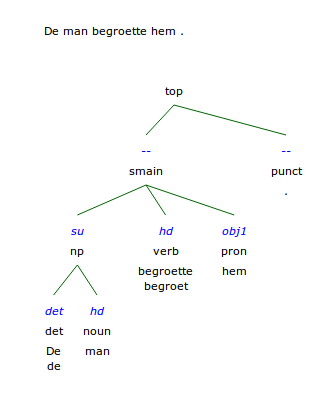
\includegraphics[width=60.0mm]{alpino.png}
\end{center}
\caption{Alpino dependency parse for the Dutch sentence ``De man begroette hem.''}
\label{fig:depparse} 
\end{figure}
\FloatBarrier

\begin{lstlisting}[language=xml]
<s xml:id="example.p.1.s.1">
  <t>De man begroette hem.</t>
  <w xml:id="example.p.1.s.1.w.1"><t>De</t></w>
  <w xml:id="example.p.1.s.1.w.2"><t>man</t></w>
  <w xml:id="example.p.1.s.1.w.3"><t>begroette</t></w>
  <w xml:id="example.p.1.s.1.w.4"><t>hem</t></w>
  <w xml:id="example.p.1.s.1.w.5"><t>.</t></w>
  <syntax>
    <su xml:id="example.p.1.s.1.su.1" class="top">     
        <su xml:id="example.p.1.s.1.su.1_1" class="smain">     
            <su xml:id="example.p.1.s.1.su.1_1_1" class="np">     
                <su xml:id="example.p.1.s.1.su.1_1_1_1" class="top">     
                    <wref id="example.p.1.s.1.w.1" t="De" />       
                </su>
                <su xml:id="example.p.1.s.1.su.1_1_1_2" class="top">     
                    <wref id="example.p.1.s.1.w.2" t="man" />
                </su> 
            </su>
            <su xml:id="example.p.1.s.1.su.1_1_2" class="verb">     
                <wref id="example.p.1.s.1.w.3" t="begroette" />   
            </su>
            <su xml:id="example.p.1.s.1.su.1_1_3" class="pron">     
                <wref id="example.p.1.s.1.w.4" t="hem" />   
            </su>
        </su>
        <su xml:id="example.p.1.s.1.su.1_2" class="punct">
            <wref id="example.p.1.s.1.w.5" t="." />               
        </su> 
    </su>
  </syntax>
  <dependencies>    
    <dependency xml:id="example.p.1.s.1.dependency.1" class="su">
        <hd>
            <wref id="example.p.1.s.1.w.3" t="begroette">
            <aref id="example.p.1.s.1.su.1_1_2" type="su">
        </hd>
        <dep>
            <wref id="example.p.1.s.1.w.2" t="man" />  
            <aref id="example.p.1.s.1.su.1_1_1" type="su">     
        </dep>
    </dependency>        
    <dependency xml:id="example.p.1.s.1.dependency.3" class="obj1">
        <hd>
            <wref id="example.p.1.s.1.w.3" t="begroette">
            <aref id="example.p.1.s.1.su.1_1_2" type="su">
        </hd>
        <dep>
            <wref id="example.p.1.s.1.w.4" t="hem" />   
            <aref id="example.p.1.s.1.su.1_1_3" type="su">
        </dep>
    </dependency>
    <dependency xml:id="example.p.1.s.1.dependency.2" class="det">
        <hd>           
           <wref id="example.p.1.s.1.w.2" t="man" />   
           <aref id="example.p.1.s.1.su.1_1_1_2" type="su">
        </hd>
        <dep>            
            <wref id="example.p.1.s.1.w.1" t="De" />   
            <aref id="example.p.1.s.1.su.1_1_1_1" type="su">
        </dep>
    </dependency>   
  </dependencies>
</s>
\end{lstlisting}


Note that in the first dependency relation, the dependant is just ``man'' rather than ``de man'' . That is, we point only to the head of dependants, the full scope follows automatically when building the dependency tree.


The declaration (the actual sets are fictitious):

\begin{lstlisting}[language=xml]
<annotations>
    <syntax-annotation 
     set="http://ilk.uvt.nl/folia/sets/alpino-syntax" /> 
    <dependency-annotation 
     set="http://ilk.uvt.nl/folia/sets/alpino-dep" />
</annotations>
\end{lstlisting}



\subsection{Chunking}

\status{final}{pynlpl,libfolia}

Unlike a full syntactic parse, chunking is not nested. The layer for this type of linguistic annotation is predictably called \texttt{chunking}. The span annotation element itself is \texttt{chunk}.

\begin{lstlisting}[language=xml]
<s xml:id="example.p.1.s.1">
  <t>The Dalai Lama greeted him.</t>
  <w xml:id="example.p.1.s.1.w.1"><t>The</t></w>
  <w xml:id="example.p.1.s.1.w.2"><t>Dalai</t></w>
  <w xml:id="example.p.1.s.1.w.3"><t>Lama</t></w>
  <w xml:id="example.p.1.s.1.w.4"><t>greeted</t></w>
  <w xml:id="example.p.1.s.1.w.5"><t>him</t></w>
  <w xml:id="example.p.1.s.1.w.6"><t>.</t></w>
  <chunking>
    <chunk xml:id="example.p.1.s.1.chunk.1">       
        <wref id="example.p.1.s.1.w.1" t="The" />       
        <wref id="example.p.1.s.1.w.2" t="Dalai" />       
        <wref id="example.p.1.s.1.w.3" t="Lama" />        
    </chunk>
    <chunk xml:id="example.p.1.s.1.chunk.2">       
        <wref id="example.p.1.s.1.w.4" t="greeted" />
    </chunk>
    <chunk xml:id="example.p.1.s.1.chunk.3">       
        <wref id="example.p.1.s.1.w.5" t="him" />
        <wref id="example.p.1.s.1.w.6" t="." />
    </chunk>    
  </chunking>
</s>
\end{lstlisting}


The declaration (the actual sets are fictitious):

\begin{lstlisting}[language=xml]
<annotations>
    <chunking-annotation 
     set="http://ilk.uvt.nl/folia/sets/syntax-nl" />
</annotations>
\end{lstlisting}

\subsection{Time Segmentation}
\label{sec:timesegment}

\status{final since v0.8, renamed in v0.9}{pynlpl}

FoLiA supports time segmentation using the \texttt{timing} layer and the \texttt{timesegment} span annotation element. This element is useful for  speech, but can also be used for event annotation. We already saw events as structure annotation in Section~\ref{sec:events}, but for more fine-grained control of timing information a span annotation element in an offset layer is more suited. The following example illustrates the usage for event annotation:

\begin{lstlisting}[language=xml]
<s>
 <w xml:id="example.p.1.s.1.w.1"><t>I</t></w>
 <w xml:id="example.p.1.s.1.w.2"><t>think</t></w>
 <w xml:id="example.p.1.s.1.w.3"><t>I</t></w>
 <w xml:id="example.p.1.s.1.w.4"><t>have</t></w>
 <w xml:id="example.p.1.s.1.w.5"><t>to</t></w>
 <w xml:id="example.p.1.s.1.w.6"><t>go</t></w>
 <w xml:id="example.p.1.s.1.w.7"><t>.</t></w>
 <timing>
  <timesegment class="utterance" begindatetime="2011-12-15T19:01" 
   enddatetime="2011-12-15T19:03" actor="myself">
    <wref id="example.p.1.s.1.w.1" t="I" />
    <wref id="example.p.1.s.1.w.2" t="think" />
  </timesegment>
  <timesegment class="cough" begintime="2011-12-15T19:03" 
   endtime="2011-12-15T19:05" actor="myself">   
  </timesegment>
  <timesegment class="utterance" begindatetime="2011-12-15T19:05" 
   enddatetime="2011-12-15T19:06" actor="myself">
    <wref id="example.p.1.s.1.w.3" t="I" />
    <wref id="example.p.1.s.1.w.4" t="have" />
    <wref id="example.p.1.s.1.w.5" t="to" />
    <wref id="example.p.1.s.1.w.6" t="go" />
  </timesegment>
 </timing>
</s>
\end{lstlisting}


Time segments may also be nested. As always, the classes in the example are set-defined rather than predefined by FoLiA. The prefefined and optional features \texttt{begindatetime} and \texttt{enddatetime} can be used express the exact moment at which an event started or ended. These too are set-defined so the format shown here is just an example.



The declaration for time segmentation is as follows:

\begin{lstlisting}[language=xml]
<annotations>
    <timesegment-annotation
     set="http://ilk.uvt.nl/folia/sets/events" />
</annotations>
\end{lstlisting}


If you are only interested in an annotation of events, and a coarser level of annotation suffices, then use the structure annotation element \texttt{event} instead. See Section~\ref{sec:events}.


\textbf{Note:} Time segments were known as "timed events" in FoLiA 0.8 and below. They have been renamed to a more appropriate and more generic name. For backward compatibility, libraries should implement \texttt{timedevent} as an alias for \texttt{timesegment}, and \texttt{timedevent-annotation} as an alias for \texttt{timesegment-annotation}.


\subsubsection{Time segmentation in a speech context}

\status{PROPOSED in v0.9}{pynlpl}

If used in a speech context, all the generic speech attributes become available (See Section~\ref{sec:speech}). This introduces  \texttt{begintime} and \texttt{endtime}, which are different from \texttt{begindatetime} and \texttt{enddatetime} ! The generic attributes \texttt{begintime} and \texttt{endtime} are not defined by the set, but specify a time location in HH:MM:SS.MMMM format which may refer to the location in an associated sound file. Sound files are associated using the \texttt{src} attribute, which is inherited by all lower elements, so we put it on the sentence here:

\begin{lstlisting}[language=xml]
<s src="ithinkihavetogo.mp3">
 <w xml:id="example.p.1.s.1.w.1"><t>I</t></w>
 <w xml:id="example.p.1.s.1.w.2"><t>think</t></w>
 <w xml:id="example.p.1.s.1.w.3"><t>I</t></w>
 <w xml:id="example.p.1.s.1.w.4"><t>have</t></w>
 <w xml:id="example.p.1.s.1.w.5"><t>to</t></w>
 <w xml:id="example.p.1.s.1.w.6"><t>go</t></w>
 <w xml:id="example.p.1.s.1.w.7"><t>.</t></w>
 <timing>
  <timesegment begintime="00:00:00.0000" 
   endtime="00:00:00.2500">
    <wref id="example.p.1.s.1.w.1" t="I" />
  </timesegment>
  <timesegment begintime="00:00:00.2500" 
   endtime="00:00:00.5000">
    <wref id="example.p.1.s.1.w.2" t="think" />
  </timesegment>
  <timesegment begintime="00:00:00.5000" 
   endtime="00:00:00.7500">
    <wref id="example.p.1.s.1.w.3" t="I" />
  </timesegment>
  <timesegment begintime="00:00:00.7500" 
   endtime="00:00:01.000">
    <wref id="example.p.1.s.1.w.4" t="have" />
  </timesegment>
  <timesegment begintime="00:00:01.0000" 
   endtime="00:00:01.250">
    <wref id="example.p.1.s.1.w.5" t="to" />
  </timesegment>
  <timesegment begintime="00:00:01.2500" 
   endtime="00:00:01.5000">
    <wref id="example.p.1.s.1.w.6" t="go" />
  </timesegment>
 </timing>
</s>
\end{lstlisting}

In a speech context, all structural elements may carry the generic attributes. So the time segmentation in the previous example, though valid, is not the most intuitive way of accomplishing this. Instead, time segmentation can better be used when actual classes are assigned:

\begin{lstlisting}[language=xml]
<s src="ithinkihavetogo.mp3">
 <w xml:id="example.p.1.s.1.w.1"
  begintime="00:00:00.0000" endtime="00:00:00.2500"><t>I</t></w>
 <w xml:id="example.p.1.s.1.w.2"
  begintime="00:00:00.2500" endtime="00:00:00.5000"><t>think</t></w>
 <w xml:id="example.p.1.s.1.w.3" 
  begintime="00:00:00.5000" endtime="00:00:00.7500"><t>I</t></w>
 <w xml:id="example.p.1.s.1.w.4"
  begintime="00:00:00.7500" endtime="00:00:01.0000"><t>have</t></w>
 <w xml:id="example.p.1.s.1.w.5" 
  begintime="00:00:01.0000" endtime="00:00:01.2500"><t>to</t></w>
 <w xml:id="example.p.1.s.1.w.6" 
  begintime="00:00:01.2500" endtime="00:00:01.5000"><t>go</t></w>
 <w xml:id="example.p.1.s.1.w.7"><t>.</t></w>
 <timing>
	<timesegment class="emphasised">
		<wref id="example.p.1.s.1.w.3" />
		<wref id="example.p.1.s.1.w.4" />
		<wref id="example.p.1.s.1.w.5" />
		<wref id="example.p.1.s.1.w.6" />
	</timesegment>
 </timing>
</s>
\end{lstlisting}

This usage, and the freedom FoLiA sets offer, opens up possibilities for a wide variety of time-segmented annotations. Moreover, the wref element does not necessarily point at words, but it may also point at phonemes. This will be introduced in Section~\ref{sec:phonemes}.

 
\subsection{Semantic Roles}

\status{new in 0.9}{pynlpl}

Semantic roles, or thematic roles, are implemented in FoLiA using the span-annotation element \texttt{semrole}, within the annotation layer \texttt{semroles}, usually embedded at sentence level.

\begin{lstlisting}[language=xml]
<s xml:id="example.p.1.s.1">
  <t>The Dalai Lama greeted him.</t>
  <w xml:id="example.p.1.s.1.w.1"><t>The</t></w>
  <w xml:id="example.p.1.s.1.w.2"><t>Dalai</t></w>
  <w xml:id="example.p.1.s.1.w.3"><t>Lama</t></w>
  <w xml:id="example.p.1.s.1.w.4"><t>greeted</t></w>
  <w xml:id="example.p.1.s.1.w.5"><t>him</t></w>
  <w xml:id="example.p.1.s.1.w.6"><t>.</t></w>
  <semroles>
	<semrole class="agent">
		<wref id="example.p.1.s.1.w.2" />
		<wref id="example.p.1.s.1.w.3" />
	</semrole>
	<semrole class="patient">
		<wref id="example.p.1.s.1.w.5" />
	</semrole>
  </semroles>
</s>
\end{lstlisting}

Semantic roles commonly correspond with syntactic units. Links between the two can be expressed using FoLiA's facility for alignments (see also Section~\ref{sec:alignments}), which were already seen in dependency relations as well. The \texttt{aref} element may be used from within the \texttt{semrole} element to link to a syntactic unit, or anything else for that matter. The following example illustrates this:

\begin{lstlisting}[language=xml]
<s xml:id="example.p.1.s.1">
  <t>De man begroette hem.</t>
  <w xml:id="example.p.1.s.1.w.1"><t>De</t></w>
  <w xml:id="example.p.1.s.1.w.2"><t>man</t></w>
  <w xml:id="example.p.1.s.1.w.3"><t>begroette</t></w>
  <w xml:id="example.p.1.s.1.w.4"><t>hem</t></w>
  <w xml:id="example.p.1.s.1.w.5"><t>.</t></w>
  <syntax>
    <su xml:id="example.p.1.s.1.su.1" class="top">     
        <su xml:id="example.p.1.s.1.su.1_1" class="smain">     
            <su xml:id="example.p.1.s.1.su.1_1_1" class="np">     
                <su xml:id="example.p.1.s.1.su.1_1_1_1" class="top">     
                    <wref id="example.p.1.s.1.w.1" t="De" />       
                </su>
                <su xml:id="example.p.1.s.1.su.1_1_1_2" class="top">     
                    <wref id="example.p.1.s.1.w.2" t="man" />
                </su> 
            </su>
            <su xml:id="example.p.1.s.1.su.1_1_2" class="verb">     
                <wref id="example.p.1.s.1.w.3" t="begroette" />   
            </su>
            <su xml:id="example.p.1.s.1.su.1_1_3" class="pron">     
                <wref id="example.p.1.s.1.w.4" t="hem" />   
            </su>
        </su>
        <su xml:id="example.p.1.s.1.su.1_2" class="punct">
            <wref id="example.p.1.s.1.w.5" t="." />               
        </su> 
    </su>
  </syntax>
  <semroles>
	<semrole class="agent">
		<wref id="example.p.1.s.1.w.1" />
		<wref id="example.p.1.s.1.w.2" />
		<aref id="example.p.1.s.1.su.1_1_1" type="su">
	</semrole>
	<semrole class="patient">
		<wref id="example.p.1.s.1.w.4" />
		<aref id="example.p.1.s.1.su.1_1_3" type="su">
	</semrole>
  </semroles>
</s>
\end{lstlisting}

The \texttt{hd} element can optionally be used to mark the head of a semantic role:

\begin{lstlisting}[language=xml]
	<semrole class="agent">
		<wref id="example.p.1.s.1.w.1" t="de" />
		<hd>
			<wref id="example.p.1.s.1.w.2" t="man" />
		</hd>
		<aref id="example.p.1.s.1.su.1_1_2" type="su">
	</semrole>
\end{lstlisting}

The mandatory declaration for semantic role annotation is as follows:

\begin{lstlisting}[language=xml]
<annotations>
    <semrole-annotation set="http://ilk.uvt.nl/folia/sets/semroles" />
</annotations>
\end{lstlisting}

\subsection{Coreference Relations}
\label{sec:coref}

\status{new in 0.9}{pynlpl}

Relations between words that refer to the same referent are expressed in FoLiA using the \texttt{coreferencechain} and \texttt{coreferencelink} span-annotation elements, within the \texttt{coreferences} annotation layer. This is done by specifying the entire chain in which all links are coreferent. The head of a coreference may optionally be marked with the \texttt{hd} element. This annotation layer itself may be embedded on whatever level is preferred. The following example uses paragraph level, but you can for instance also embed it at sentence level or a global text level:  

\begin{lstlisting}[language=xml]
<p xml:id="example.p.1">
<s xml:id="example.p.1.s.1">
  <t>The Dalai Lama greeted him.</t>
  <w xml:id="example.p.1.s.1.w.1"><t>The</t></w>
  <w xml:id="example.p.1.s.1.w.2"><t>Dalai</t></w>
  <w xml:id="example.p.1.s.1.w.3"><t>Lama</t></w>
  <w xml:id="example.p.1.s.1.w.4"><t>greeted</t></w>
  <w xml:id="example.p.1.s.1.w.5"><t>him</t></w>
  <w xml:id="example.p.1.s.1.w.6"><t>.</t></w>
</s>
<s xml:id="example.p.1.s.2">
  <t>He was happy to see him.</t>
  <w xml:id="example.p.1.s.2.w.1"><t>He</t></w>
  <w xml:id="example.p.1.s.2.w.2"><t>was</t></w>
  <w xml:id="example.p.1.s.2.w.3"><t>happy</t></w>
  <w xml:id="example.p.1.s.2.w.4"><t>to</t></w>
  <w xml:id="example.p.1.s.2.w.4"><t>see</t></w>
  <w xml:id="example.p.1.s.2.w.5"><t>him</t></w>
  <w xml:id="example.p.1.s.2.w.6"><t>.</t></w>  
</s>
<s xml:id="example.p.1.s.3">
  <t>He smiled.</t>
  <w xml:id="example.p.1.s.3.w.1"><t>He</t></w>
  <w xml:id="example.p.1.s.3.w.2"><t>smiled</t></w>
  <w xml:id="example.p.1.s.3.w.3"><t>.</t></w>
</s>
<coreferences>
    <coreferencechain class="ident">
      <coreferencelink>
          <wref id="example.p.1.s.1.w.1" t="The" />
          <hd>
            <wref id="example.p.1.s.1.w.2" t="Dalai" />
            <wref id="example.p.1.s.1.w.3" t="Lama" />
          </hd>
      </coreferencelink>
      <coreferencelink>
        <wref id="example.p.1.s.2.w.1" t="he" />
      </coreferencelink>
    </coreferencechain>
    <coreferencechain class="ident">
      <coreferencelink>
        <wref id="example.p.1.s.2.w.5" t="him" />
      </coreferencelink>
      <coreferencelink>
        <wref id="example.p.1.s.2.w.6" t="him" />
      </coreferencelink>
      <coreferencelink>
        <wref id="example.p.1.s.3.w.1" t="He" />
      </coreferencelink>
    </coreferencechain>
</coreferences>
</p>
\end{lstlisting}

Being a span-annotation element, the \texttt{coreference} element may take all of the usual attributes. Most notable is the \texttt{class} element designating the type of coreference relation. Like its parent, each of the links in the chain may take the standard attributes \texttt{annotator}, \texttt{annotatortype}, \texttt{datetime}, \texttt{confidence}. The links or heads do not take a class, only \texttt{coreferencechain} does.

\texttt{Coreferencelink} may take three attributes, which are actually predefined FoLiA subsets (See Section~\ref{sec:features}), their values depend on the set used and are thus user-definable and never predefined: 

\begin{itemize} %As suggested by Orphee De Clerq
\item \texttt{modality} - A subset that can be used for indication that there is modality or negation in this coreference link.
\item \texttt{time} - A subset used to indicate a time dependency. An example of a time dependency is seen in the sentence: ``Bert De Graeve, until recently CEO, will now take up a position as CFO''. Here 
``Bert De Graeve'', ``CEO''  and ``CFO'' would all be part of the same coreference chain, and the second \texttt{coreferencelink} (``CEO'') can be marked as being in the past using the ``time'' attribute.
\item \texttt{level} - A subset used that can indicate the level on which the coreference holds. A possible value suggestion could be ``sense'', indicating that only on sense-level there is a corefence relation, as opposed to an actual reference.
\end{itemize}

%TODO: more examples?

The declaration for coreference relations is done as follows:

\begin{lstlisting}[language=xml]
<annotations>
    <coreference-annotation 
     set="http://ilk.uvt.nl/folia/sets/coref" />
</annotations>
\end{lstlisting}

\section{Morphological Annotation}

\status{heavily revised since v0.9}{pynlpl}

Tokens can be further segmented into morphemes, a form of structure annotation. Morphemes behave much like \texttt{w} elements (tokens). Moreover, morphemes can be referred to from within in span annotation using \texttt{wref}, allowing spans to be defined not only over whole words/tokens but also parts thereof. The element for morphemes is \texttt{morpheme}, and can only occur within \texttt{w} elements. Recall that \texttt{t} elements can contain references to higher-level \texttt{t} elements. In such cases, the \texttt{offset} attribute is used to designate the offset index in the word's associated text element (\texttt{t}) (zero being right at the start of the text). Morphemes may do this.

Furthermore, a morpheme may take a class, referring to its type. As always, the classes are defined by the declared set, and not predefined by the FoLiA set. Declaration proceeds as follows, the actual set is fictitious:

\begin{lstlisting}[language=xml]
<annotations>
    <morphology-annotation 
     set="http://ilk.uvt.nl/folia/sets/morphology" />
</annotations>
\end{lstlisting}

Morphemes are grouped in a \texttt{morphology} layer, which itself takes no attributes. An example of morphology in use:

\begin{lstlisting}[language=xml]
<w xml:id="example.p.4.s.2.w.4">
    <t>leest</t>
    <lemma class="lezen" />
    <morphology>
        <morpheme class="stem" function="lexical">
            <t offset="0">lees</t>
        </morpheme>
        <morpheme class="suffix" function="inflexional">
            <t offset="4">t</t>
        </morpheme>
    </morphology>
</w>
\end{lstlisting}

Note that the attribute \texttt{function} is a predefined feature you may use (not mandatory), its values are defined by the set rather than the FoLiA standard, so they are user/set-defined.

Morphemes allow token annotation just as words do. We can for instance bind lemma annotation to the morpheme representing the word's stem rather than only to the entire word:

\begin{lstlisting}[language=xml]
<w xml:id="example.p.4.s.2.w.4">
    <t>leest</t>
    <lemma class="lezen" />
    <morphology>
        <morpheme xml:id="example.p.4.s.2.w.4.m.1" class="stem" 
         function="lexical">
			<lemma class="lezen" />
            <t offset="0">lees</t>
        </morpheme>
        <morpheme xml:id="example.p.4.s.2.w.4.m.2" class="suffix"
         function="inflexional">
            <t offset="4">t</t>
        </morpheme>
    </morphology>
</w>
\end{lstlisting}

Similarly, consider the Spanish word or phrase ``D\'amelo'' (give it to me),
written as one entity. If this has not been split during tokenisation, but left
as a single token, you can annotate its morphemes, as all morphemes allow token
annotation to be placed within their scope:

\begin{lstlisting}[language=xml]
<w xml:id="example.p.1.s.1.w.1">
    <t>dámelo</t>
    <morphology>
        <morpheme class="stem">
            <t offset="0">dá</t>
			<lemma class="dar" />
			<pos class="v" />
        </morpheme>
        <morpheme class="suffix">
            <t offset="2">me</t>
			<lemma class="me" />
			<pos class="pron" />
        </morpheme>
        <morpheme class="suffix">
            <t offset="4">lo</t>
			<lemma class="lo" />
			<pos class="pron" />
        </morpheme>
    </morphology>
</w>
\end{lstlisting}

Unlike words, morphemes may also be nested, as they can be expressed on multiple levels:

\begin{lstlisting}[language=xml]
<w xml:id="example.p.1.s.1.w.1">
    <t>comfortable</t>
    <morphology>
        <morpheme class="base">
            <t offset="0">comfort</t>
			<morpheme class="prefix">
				<t offset="0">com</t>
			</morpheme>
			<morpheme class="morph">
				<t offset="3">fort</t>				
			</morpheme>
        </morpheme>
        <morpheme class="suffix">
            <t offset="7">able</t>
        </morpheme>
    </morphology>
</w>
\end{lstlisting}


Note that the annotation of morphology has changed since FoLiA version 0.9. Older versions did not yet assign a class to morphemes themselves, but rather only used features, which were entirely left to the set to define. These documents remain valid in FoLiA 0.9 and above, but this way is no longer the recommended way. The following example illustrates the old style:

\begin{lstlisting}[language=xml]
<w xml:id="example.p.4.s.2.w.4">
    <t>leest</t>
    <lemma class="lezen" />
    <morphology>
        <morpheme>
            <feat subset="type" class="stem">
            <feat subset="function" class="lexical">
            <t offset="0">lees</t>
        </morpheme>
        <morpheme>
            <feat subset="type" class="suffix">
            <feat subset="function" class="inflexional">
            <t offset="4">t</t>
        </morpheme>
    </morphology>
</w>
\end{lstlisting}


The next example will illustrate how morphemes can be referred to in span annotation. Here we have a morpheme, and not the entire word, which forms a named entity:

\begin{lstlisting}[language=xml]
<w xml:id="example.p.4.s.2.w.4">
    <t>CDA-voorzitter</t>
    <morphemes>
		<morpheme xml:id="example.p.4.s.2.w.1.m.1">
			<t offset="0">CDA</t>
		</morpheme>
	</morphemes>	
	<entities>
		<entity xml:id="entity.1">
			<wref id="example.p.4.s.2.w.1.m.1" />
		</entity>
	</entities>
</w>
\end{lstlisting}

The older FoLiA elements \texttt{subentities} and \texttt{subentity} are deprecated in favour of this new approach.

The same approach can be followed for other kinds of span annotation. Note that the span annotation layer (\texttt{entities} in the example) may be embedded on various levels. Most commonly on sentence level, but also on word level, paragraph level or the global text level.

%\subsection{Named Entities within a token}

%\status{final since v0.4}{pynlpl,libfolia}

%Named entities may sometimes occur as \emph{part} of a token. The \texttt{subentities} annotation layer and the \texttt{subentity} subtoken annotation element can be used for annotating these:  

%\begin{lstlisting}[language=xml]
%<w xml:id="example.p.4.s.2.w.4">
%    <t>CDA-voorzitter</t>
 %   <subentities>
 %       <subentity class="org" annotator="Maarten van Gompel"
 %           annotatortype="manual">
 %           <t offset="0">CDA</t>
 %       </subentity>
 %   </subentities>
%</w>
%\end{lstlisting}

%The declaration:

%\begin{lstlisting}[language=xml]
%<annotations>
%    <subentity-annotation set="http://ilk.uvt.nl/folia/sets/entities" />
%</annotations>
%\end{lstlisting}

\section{Speech Annotation}

\status{Proposed in v0.9}{not implemented yet}

\subsection{Speech Structure Annotation}
\label{sec:speech}

\status{Proposed in v0.9}{not implemented yet}

FoLiA is not just suited for the annotation of text, but also accommodates annotation of transcribed speech. This generally asks for a different document structure than text documents. The top-level element for speech-centred resources is \texttt{speech}. Certain elements described in the section on text structure may be used under \texttt{speech} as well; such as divisions (\texttt{div}), sentences (\texttt{s)} and words (\texttt{w}). Notions such as paragraphs and figures make less sense in a speech context.

All structure elements in a speech context may take the extra FoLiA attributes for speech, as laid out in Section~\ref{sec:speechparadigm}. These include attributes for referring to associating sound clips.

\subsubsection{Utterances}

\status{Proposed in v0.9}{not implemented yet}


An utterance may consist of words or sentences, which in turn may contain words. The opposite is also true, a sentence may consist of multiple utterances. The utterance element in FoLiA is \texttt{utt}. 

Utterances need not be declared necessarily, but may be if classes are assigned. The actual set in the example is fictitious:

\begin{lstlisting}[language=xml]
<annotations>
    <utterance-annotation 
     set="http://ilk.uvt.nl/folia/sets/utterances" />
</annotations>
\end{lstlisting}

An actual example of utterances is shown later in the section on phonetic content.

\subsubsection{Non-speech events}

Non-speech events are simply covered by \texttt{event} annotation as seen in Section \ref{sec:events}. Consider the following small example, with speech-context attributes associated:

\begin{lstlisting}[language=xml]
<event class="cough" src="soundclip.mp3"
 begintime="..." endtime="..." />
\end{lstlisting}

\subsection{Phonetic Content}

\status{Proposed in v0.9}{not implemented yet}

Written text is always contained in the text content element (\texttt{t}), for phonetics there is a similar counterpart: \texttt{ph}. The \texttt{ph} element holds a phonetic transcription. It is used in a very similar fashion:

\begin{lstlisting}[language=xml]
<utt src="helloworld.mp3"  begintime="..." endtime="...">
	<ph>helˈoʊ wɝːld</ph>
	<w xml:id="example.utt.1.w.1" 
     begintime="..." endtime="...">
		<ph>helˈoʊ</ph>	
	</w>
	<w xml:id="example.utt.1.w.2"  
     begintime="..." endtime="...">
		<ph>wɝːld</ph>	
	</w>
</utt>
\end{lstlisting}

Like the \texttt{t} element, the \texttt{ph} element supports the \texttt{offset} attribute, referring to the offset in the phonetic transcription. The first index being zero. Phonetic transcription and text content can also go together without problem:

\begin{lstlisting}[language=xml]
<utt>
	<ph>helˈoʊ wɝːld</ph>
	<t>hello world</t>
	<w xml:id="example.utt.1.w.1">
		<ph offset="0">helˈoʊ</ph>
		<t offset="0">hello</t>	
	</w>
	<w xml:id="example.utt.1.w.2">
		<ph offset="8">wɝːld</ph>
		<t offset="6">world</t>	
	</w>
</utt>
\end{lstlisting}

\subsection{Phoneme Annotation}
\label{sec:phonemes}

\status{PROPOSED in v0.9}{not implemented yet}

The smallest unit of annotatable speech in FoLiA is the phoneme level. The \texttt{phoneme} element is a form of structure annotation used for phonemes. Alike to morphology, it is embedded within a layer \texttt{phonetics} which can be used within word/token elements (\texttt{w}) or directly within \texttt{utt} if no words are distinguished:


\begin{lstlisting}[language=xml]   
<utt>
  <w xml:id="word" src="book.wav">
    <t>book</t>
    <ph>bʊk</ph>
    <phonetics>
      <phoneme begintime="..."  endtime="...">
          <ph>b</ph>
      </phoneme>
      <phoneme begintime="..." endtime="...">
          <ph>ʊ</ph>
      </phoneme>
      <phoneme begintime="..." endtime="...">
          <ph>k</ph>
      </phoneme>
    </phonetics>
  </w>
</utt>
\end{lstlisting}

Phoneme annotation needs to be declared if classes are assigned to the phonemes:

\begin{lstlisting}[language=xml]
<annotations>
    <phoneme-annotation 
     set="http://ilk.uvt.nl/folia/sets/utterances" />
</annotations>
\end{lstlisting}


\subsection{Distortion}

\status{Proposed in v0.9}{not implemented yet}


FoLiA has a token annotation element \texttt{distortion} which can be used in a speech context. It indicates that a certain distortion of change in the sound speech has taken place. It can be used for background sounds. The classes are of course not predefined by the FoLiA format but depend on the class used:

\begin{lstlisting}[language=xml]
<utt>
	<ph>helˈoʊ wɝːld</ph>
	<distortion class="windnoise" />
</utt>
\end{lstlisting}

The distortion element is also useful to mark specific accents or dialects, depending of course on the set used:

\begin{lstlisting}[language=xml]
<utt>
	<t>day</t>
	<ph>dæi</ph>
	<distortion class="cockney" />
</utt>
\end{lstlisting}

The mandatory declaration goes as follows (the set is fictitious):

\begin{lstlisting}[language=xml]
<annotations>
    <distortion-annotation 
     set="http://ilk.uvt.nl/folia/sets/distortion" />
</annotations>
\end{lstlisting}









\section{Higher-order Annotation}
\label{sec:higherorder}

We introduced the FoLiA paradigm in Section~\ref{sec:paradigm} and listed the four categories of annotation: structure annotation, token annotation, span annotation and higher-order annotation. In this section we will discuss the higher-order annotation elements and the more advanced aspects of  FoLiA. The higher-order annotation category forms less of a unity than the other categories. All annotations in this category have in common that they all are annotations about other annotations, relating to other annotations, or enhancing other annotations.

In our discussion of the various types of higher-order annotation, we will encounter the more advanced aspects of the FoLiA paradigm.

\subsection{Human-readable Descriptions}

\status{final since v0.6}{pynlpl,libfolia}

This is one of the simplest forms of higher-order annotation. Any annotation element may hold a \texttt{desc} element containing in its body a human readable description for the annotation. An example of this has been already shown for the \texttt{sense} and \texttt{gap} elements

\begin{lstlisting}[language=xml]
<w xml:id="example.p.1.s.1.w.1">
	<t>boot</t>
	<pos class="n">
		<desc>Noun</desc>
	</pos>	
	<desc>boot</desc>
</w>
\end{lstlisting}

\subsection{Alternative Token Annotations}
\label{sec:alternatives}

\status{final}{pynlpl,libfolia}

The FoLiA format does not just allow for a single authoritative annotation per token; it allows the representation of \emph{alternative} annotations. Alternative token annotations are grouped within one or more \texttt{alt} elements. If multiple annotations are grouped together under the same \texttt{alt} element, then they are deemed \emph{dependent} and form a single set of alternatives.

Each alternative preferably is given a unique identifier. In the following example we see the Dutch word ``bank'' in the sense of a sofa, alternatively we see two alternative annotations with a different sense and domain. Any annotation element within an \emph{alt} block by definition needs to be marked as non-authoritative by setting \texttt{auth="no"}. This facilitates the job of parsers and queriers.

\begin{lstlisting}[language=xml]
<w xml:id="example.p.1.s.1.w.1">
    <t>bank</t>
    <domain class="furniture" />
    <sense class="r_n-5918" synset="d_n-21410" 
     annotator="John Doe" annotatortype="manual" 
     confidence="1.0">zitmeubel</sense>
    <alt xml:id="example.p.1.s.1.w.1.alt.1">
        <domain auth="no" class="finance" />
        <sense auth="no" class="r_n-5919" synset="d_n-27025"
         annotator="Jane Doe" annotatortype="manual" 
         confidence="0.6">geldverlenende instelling</sense>        
    </alt>
    <alt xml:id="example.p.1.s.1.w.1.alt.2">
        <domain auth="no" class="geology" />
        <sense auth="no" class="r_n-5920" synset="d_n-38257"
         annotator="Jim Doe" annotatortype="manual"
         confidence="0.1">zandbank</sense>        
    </alt>    
</w>
\end{lstlisting}


Sometimes, an alternative is concerned only with a portion of the annotations.
By default, annotations not mentioned are applicable to the alternative as
well, unless the alternative is set as being \emph{exclusive}. Consider the
following expanded example in which we added a part-of-speech tag and a lemma.

\begin{lstlisting}[language=xml]
<w xml:id="example.p.1.s.1.w.1">
    <t>bank</t>
    <domain class="furniture" />
    <sense class="r_n-5918" synset="d_n-21410" 
     annotator="John Doe" annotatortype="manual" 
     confidence="1.0">furniture</sense>
    <pos class="n" />
    <lemma class="bank" />
    <alt xml:id="example.p.1.s.1.w.1.alt.1">
        <domain auth="no" class="finance" />
        <sense auth="no" class="r_n-5919" synset="d_n-27025"
         annotator="Jane Doe" annotatortype="manual" 
         confidence="0.6">financial institution</sense>        
    </alt>
    <alt xml:id="example.p.1.s.1.w.1.alt.2">
        <domain auth="no" class="geology" />
        <sense auth="no" class="r_n-5920" synset="d_n-38257"
         annotator="Jim Doe" annotatortype="manual"
         confidence="0.1">river bank</sense>        
    </alt>    
    <alt xml:id="example.p.1.s.1.w.1.alt.2" exclusive="yes">
		<t>bank</t>
        <domain auth="no" class="navigation" />
        <sense auth="no" class="r_n-1234">to turn</sense>        
		<pos class="v" />
	    <lemma class="bank" />
    </alt>    
</w>
\end{lstlisting}

The first two alternatives are inclusive, which is the default. This means that
the pos tag ``n'' and the lemma ``bank'' apply to them as well. The last
alternative is set as exclusive, using the \texttt{exclusive} attribute. It has
been given a different pos tag and the lemma and even the text content have
been repeated even though they are equal to the higher-level annotation,
otherwise there would be no lemma nor text associated with the exclusive
alternative.

Alternatives can be used as a great way of postponing actual annotation, due to their non-authoritative nature. When used in this way, they can be regarded as ``options''. They can be used even when there are no authoritative annotations of the type.  Consider the following example in which domain and sense annotations are presented as alternatives and there is no authoritative annotation of these types whatsoever:

\begin{lstlisting}[language=xml]
<w xml:id="example.p.1.s.1.w.1">
    <t>bank</t>
    <alt xml:id="example.p.1.s.1.w.1.alt.1">
        <domain auth="no" class="finance" />
        <sense auth="no" class="r_n-5919" synset="d_n-27025"
         annotator="Jane Doe" annotatortype="manual" 
         confidence="0.6">geldverlenende instelling</sense>        
    </alt>
    <alt xml:id="example.p.1.s.1.w.1.alt.2">
        <domain auth="no" class="geology" />
        <sense auth="no" class="r_n-5920" synset="d_n-38257"
         annotator="Jim Doe" annotatortype="manual"
         confidence="0.1">zandbank</sense>        
    </alt>    
</w>
\end{lstlisting}

\subsection{Alternative Span Annotations}

With token annotations one can specify an unbounded number of alternative annotations. This functionality is available for span annotations as well, but due to the different nature of span annotations this happens in a slightly different way.

Where we used \texttt{alt} for token annotations, we now use \texttt{altlayers} for span annotations. Under this element several alternative layers can be presented. Analogous to \texttt{alt}, any layers grouped together are assumed to be somehow dependent. Multiple \texttt{altlayers} can be added to introduce independent alternatives. Each alternative may be associated with a unique identifier. The layers within \texttt{altlayers} need to be marked as non-autoritative using \texttt{auth="no"}.

Below is an example of a sentence that is chunked in two ways:

\begin{lstlisting}[language=xml]
<s xml:id="example.p.1.s.1">
  <t>The Dalai Lama greeted him.</t>
  <w xml:id="example.p.1.s.1.w.1"><t>The</t></w>
  <w xml:id="example.p.1.s.1.w.2"><t>Dalai</t></w>
  <w xml:id="example.p.1.s.1.w.3"><t>Lama</t></w>
  <w xml:id="example.p.1.s.1.w.4"><t>greeted</t></w>
  <w xml:id="example.p.1.s.1.w.5"><t>him</t></w>
  <w xml:id="example.p.1.s.1.w.6"><t>.</t></w>
  <chunking>
    <chunk xml:id="example.p.1.s.1.chunk.1">       
        <wref id="example.p.1.s.1.w.1" t="The" />       
        <wref id="example.p.1.s.1.w.2" t="Dalai" />       
        <wref id="example.p.1.s.1.w.3" t="Lama" />        
    </chunk>
    <chunk xml:id="example.p.1.s.1.chunk.2">       
        <wref id="example.p.1.s.1.w.4" t="greeted" />
    </chunk>
    <chunk xml:id="example.p.1.s.1.chunk.3">       
        <wref id="example.p.1.s.1.w.5" t="him" />
        <wref id="example.p.1.s.1.w.6" t="." />
    </chunk>    
  </chunking>
  <altlayers xml:id="example.p.1.s.1.alt.1">
       <chunking annotator="John Doe" 
        annotatortype="manual" confidence="0.0001" auth="no">
        <chunk xml:id="example.p.1.s.1.alt.1.chunk.1">       
            <wref id="example.p.1.s.1.w.1" t="The" />       
            <wref id="example.p.1.s.1.w.2" t="Dalai" />                       
        </chunk>
        <chunk xml:id="example.p.1.s.1.alt.1.chunk.2">       
            <wref id="example.p.1.s.1.w.2" t="Lama" />                       
            <wref id="example.p.1.s.1.w.4" t="greeted" />
        </chunk>
        <chunk xml:id="example.p.1.s.1.alt.1.chunk.3">       
            <wref id="example.p.1.s.1.w.5" t="him" />
            <wref id="example.p.1.s.1.w.6" t="." />
        </chunk>    
      </chunking>   
  </altlayers>
</s>
\end{lstlisting}

The support for alternatives and the fact that multiple layers (including those of different types) cannot be nested in a single inline structure, should make clear why FoLiA uses a stand-off notation alongside an inline notation. 


\subsection{Feature Annotation}
\label{sec:features}

\status{revised in v0.8}{pynlpl,libfolia}

In addition to a main class, an arbitrary number of \emph{features} can be added to \emph{any} annotation element. Each feature pertains to a specific \emph{subset}. Subsets and the classes within them can be invented at will as they are part of the set definition, which is left entirely to the user. However, certain annotation elements also have some predefined subsets you may use.

The element \texttt{feat} is used to add features to any kind of annotation. In the following example we make use of a subset we invented which ties a lemma to a page number in some dictionary where the lemma can be found.

\begin{lstlisting}[language=xml]
 <lemma class="house">
   <feat subset="dictionary_page" class="45" />
 </lemma>
\end{lstlisting}

A more thorough example for part-of-speech tags with features will be explained in Section~\ref{sec:posfeat}.

Some elements have predefined subsets because some features are very commonly
used. However, it still depends on the set on whether these can be used, and
which values these take. Whenever subsets are predefined in the FoLiA standard
they can be assigned using XML attributes. Consider the following example of
lexical semantic sense annotation, in which subset ``synset'' is a predefined
subset:

\begin{lstlisting}[language=xml]
<sense class="X" synset="Y" />
\end{lstlisting}

This is semantically equivalent to:

\begin{lstlisting}[language=xml]
<sense class="X">
    <feat subset="synset" class="Y" />
</sense>
\end{lstlisting}

The following example of event annotation with the feature with predefined subset ``actor'' is similar:

\begin{lstlisting}[language=xml]
<event class="tweet" actor="John Doe">
 ...
</event>
\end{lstlisting}

This is semantically equivalent to:

\begin{lstlisting}[language=xml]
<event class="tweet">
 <feat subset="actor" class="John Doe" />
 ...
</event>
\end{lstlisting}

Features can also be used to assign multiple classes within the same subset, which is impossible with main classes. In the following example the event is associated with a list of two actors. In this case the XML attribute shortcut no longer suffices, and the \texttt{feat} element must be used explicitly.

\begin{lstlisting}[language=xml]
<event class="conversation">
 <feat subset="actor" class="John Doe" />
 <feat subset="actor" class="Jane Doe" />
 <p>...</p>
</event>
\end{lstlisting}

To recap: the \texttt{feat} element can always be used freely to associate
\texttt{any} additional classes of \emph{any} designed subset with \emph{any}
annotation element. For certain elements, there are predefined subsets, in
which case you can assign them using the XML attribute shortcut. This, however,
only applies to the predefined subsets.

\subsection{Part-of-Speech Tags with Features}
\label{sec:posfeat}

\status{final}{pynlpl,libfolia}

Part-of-speech tags are a good example of the scenario outlined above.
Part-of-speech tags may consist of multiple features, which in turn \emph{may}
be associated with specific subsets. Two scenarios can be envisioned, one in
which the class of the \texttt{pos} element combines all features, and one in
which it is the foundation upon which is expanded. Which one is used is
entirely up to the defined set.

Option one:

\begin{lstlisting}[language=xml]
<w xml:id="example.p.1.s.1.w.2">
    <t>boot</t>
    <pos head="N" class="N(soort,ev,basis,zijd,stan)">
        <desc>Noun, singular, neuter</desc>
        <feat subset="ntype" class="soort" />
        <feat subset="number" class="ev" />
        <feat subset="degree" class="basis" />
        <feat subset="gender" class="zijd" />
        <feat subset="case" class="stan" />
    </pos>
</w>
\end{lstlisting}

In FoLiA, this attribute \texttt{head} is a predefined subset ``head'' of whatever set you defined. This would thus be equal to: 

\begin{lstlisting}[language=xml]
    <feat subset="head" class="N" />
\end{lstlisting}

Option two:

\begin{lstlisting}[language=xml]
<w xml:id="example.p.1.s.1.w.2">
    <t>boot</t>
    <pos class="N">
        <desc>Noun, singular, neuter</desc>
        <feat subset="ntype" class="soort" />
        <feat subset="number" class="ev" />
        <feat subset="degree" class="basis" />
        <feat subset="gender" class="zijd" />
        <feat subset="case" class="stan" />
    </pos>
</w>
\end{lstlisting}


\subsection{Metrics}

\status{final since v0.9}{pynlpl,libfolia}

The metric element allows annotation of some kind of measurement. The type of
measurement is defined by the class, which in turn is defined by the set as
always. The metric element has a \texttt{value} attribute
that stores the actual measurement, the value is often numeric but this needs
not be the case. It is a higher-level annotation element
that may be used with any kind of annotation. 

Example:

\begin{lstlisting}[language=xml]
<w xml:id="example.p.1.s.1.w.2">
    <t>boot</t>
    <metric class="charlength" value="4" />
    <metric class="frequency" value="0.00232" />
</w>
\end{lstlisting}

Example:

\begin{lstlisting}[language=xml]
<su class="np"
    <wref id="..." />
    <wref id="..." />
    <metric class="length" value="2" />
</w>
\end{lstlisting}

The declaration (the actual sets are fictitious):

\begin{lstlisting}[language=xml]
<annotations>
    <metric-annotation 
     set="http://ilk.uvt.nl/folia/sets/metrics" />
</annotations>
\end{lstlisting}


\subsection{Corrections}
\label{sec:corrections}

\status{final since v0.4}{pynlpl,libfolia}

Corrections, including but not limited to spelling corrections, can be annotated using the \texttt{correction} element. The following example shows a spelling correction of the misspelled word ``treee'' to its corrected form ``tree''.

%    <t>tree</t>
\begin{lstlisting}[language=xml]
<w xml:id="example.p.1.s.1.w.1">
    <correction xml:id="TEST-000000001.p.1.s.1.w.1.c.1" 
     class="spelling">
        <new>
            <t>tree</t>
        </new>
        <original auth="no">
            <t>treee</t>
        </original>
    </correction>
</w>
\end{lstlisting}

The class indicates the kind of correction, according to the set used. The \texttt{new} element holds the actual content of the correction. The \texttt{original} element holds the content prior to correction. Note that all corrections must carry a unique identifier. In this example, what we are correcting is the actual textual content, the text element (\texttt{t}). To facilitate the job of parsers and queriers, the original element has to be marked as being non-authoritative, using \texttt{auth="no"}. This states that this element and anything below it is not authoritative, meaning that any text or annotations within do not affect the text or annotations of the structure element (the word in this case) of which it is a part.

Corrections can be nested and we want to retain a full back-log. The following example illustrates the word ``treee'' that has been first mis-corrected to ``three'' and subsequently corrected again to ``tree'':

\begin{lstlisting}[language=xml]
<w xml:id="example.p.1.s.1.w.1">
  <correction xml:id="TEST-000000001.p.1.s.1.w.1.c.2"
    class="spelling" 
    annotator="Jane Doe" annotatortype="manual" 
    confidence="1.0">
      <new>
          <t>tree</t>
      </new>
      <original auth="no">
        <correction xml:id="TEST-000000001.p.1.s.1.w.1.c.1"
         class="spelling"
         annotator="John Doe" annotatortype="manual"
         confidence="0.6">
         <new>
             <t>three</t>
         </new>
         <original auth="no">
             <t>treee</t>
         </original>
        </correction>
      </original>
  </correction>
</w>
\end{lstlisting}

In the examples above what we corrected was the actual textual content
(\texttt{t}). However, it is also possible to correct other annotations: The
next example corrects a part-of-speech tag; in such cases, there is no
\texttt{t} element in the correction, but simply another token annotation
element, or group thereof.

\begin{lstlisting}[language=xml]
<w xml:id="example.p.1.s.1.w.1">
    <t>tree</t>
    <correction xml:id="TEST-000000001.p.1.s.1.w.1.c.1">
        <new>
            <pos class="n" />
        </new>
        <original auth="no">
            <pos class="v" />
        </original>
    </correction>
    
</w>    
\end{lstlisting}

\subsubsection{Error detection and correction with suggestions} 

\status{Revised in v0.8.2, no error attribute}{pynlpl,libfolia}

The correction of an error implies the detection of an error. In some cases, detection comes without correction, for instance when the generation of correction suggestions is postponed to a later processing stage. The \texttt{errordetection} element is a very simple element that serves this purpose. It signals the existence of errors and is a normal token annotation element: 

\begin{lstlisting}[language=xml]
<w xml:id="example.p.1.s.1.w.1">
    <t>treee</t>
    <errordetection class="spelling" annotator="errorlistX" />
</w>    
\end{lstlisting}

We can also imagine it specifically marking something as \emph{not} being an error, in which case a class could be used that denotes the absence of an error. Note that this class is in no way predefined, but always up to the user and set.

\begin{lstlisting}[language=xml]
<w xml:id="example.p.1.s.1.w.1">
    <t>tree</t>
    <errordetection class="noerror" />
</w>    
\end{lstlisting}

This kind of error detection is very simple and does not provide actual correction nor suggestions for correction. In some cases, it is desirable to record suggestions for correction, but without making the actual correction.

The correction tag can also be used in such situations in which you want to list suggestions for correction, but not yet commit to any single one. You may for example want to postponed this actual selection to another module or human annotator. Recall that the actual correction is always included in the ``new'' tag, non-committing suggestions are included in the ``suggestion'' tag. All suggestions may take an ID and may specify an annotator, if no annotator is specified it will be inherited from the \texttt{correction} element itself. Suggestions never take sets or classes by themselves, the class and set pertain to the correction as a whole, and apply to all suggestions within. This implies that you will need multiple correction elements if you want to make suggestions of very distinct types. The following example shows two suggestions for correction:
 
\begin{lstlisting}[language=xml]
<w xml:id="example.p.1.s.1.w.1">
  <t>treee</t>
  <correction xml:id="example.p.1.s.1.w.1.c.1"
      class="spelling" annotator="errorlistX">
      <suggestion confidence="0.8" auth="no">
          <t>tree</t>
      </suggestion>
      <suggestion confidence="0.2" auth="no">
          <t>three</t>
      </suggestion>
  </correction>
</w>    
\end{lstlisting}

In the situation above we have a possible correction with two suggestions, none of which has been selected yet. The actual text remains unmodified so there are no \texttt{new} or \texttt{original} tags. Note that anything in the scope of a suggestion is by definition non-authoritative and suggestions have to be marked as such using \texttt{auth="no"} to facilitate the job of parsers.

When an actual correction is made, the correction element changes. It may still retain the list of suggestions. In the following example, a human annotator named John Doe took one of the suggestions and made the actual correction:

\begin{lstlisting}[language=xml]
<w xml:id="example.p.1.s.1.w.1">
    <correction xml:id="example.p.1.s.1.w.1.c.1"
       class="spelling" annotator="John Doe"
        annotatortype="human">
        <new>
            <t>tree</t>
        </new>
        <suggestion annotator="errorlistX" auth="no"
          annotatortype="auto" confidence="0.8">
            <t>tree</t>
        </suggestion>
        <suggestion annotator="errorlistX" auth="no"
          annotatortype="auto" confidence="0.2">
            <t>three</t>
        </suggestion>
        <original auth="no">
            <t>treee</t>
        </original>
    </correction>
</w>    
\end{lstlisting}

Something similar may happen when a correction is made \emph{on the basis of} one or more kinds of error detection, the \texttt{correction} element directly embeds the \texttt{errordetection} element:

\begin{lstlisting}[language=xml]
<w xml:id="example.p.1.s.1.w.1">
    <correction class="spelling" annotator="John Doe">
        <new>
            <t>tree</t>
        </new>
        <original auth="no">
            <t>treee</t>
        </original>
        <errordetection class="spelling"
         annotator="errorlist" annotatortype="auto" />
    </correction>
</w>
\end{lstlisting}

In the above example, ``treee'' was detected by an automated error list as being an error, and was corrected to ``tree'' by human annotator John Doe.

Like everything, corrections and error detection have to be declared, and have
to be declared separately. However, nothing stops you from pointing them both
to the same set. Suggestions fall under the scope of corrections and need not
be declared separately.

\begin{lstlisting}[language=xml]
<annotations>
    <errordetection-annotation 
     set="http://ilk.uvt.nl/folia/sets/corrections" />
    <correction-annotation
     set="http://ilk.uvt.nl/folia/sets/corrections" />
</annotations>
\end{lstlisting}

\subsubsection{Merges, Splits and Swaps} 


Sometimes, one wants to merge multiple tokens into one single new token, or the other way around; split one token into multiple new ones. The FoLiA format does not allow you to simply create new tokens and reassign identifiers. Identifiers are by definition permanent and should never change, as this would break backward compatibility. So such a change is therefore by definition a correction, and one uses the \texttt{correction} tag to merge and split tokens.

We will first demonstrate a merge of two tokens (``on line'') into one (``online''). The original tokens are always retained as \texttt{w-original} elements. First a peek at the XML prior to merging:

\begin{lstlisting}[language=xml]
<s xml:id="example.p.1.s.1">
    <w xml:id="example.p.1.s.1.w.1">
        <t>on</t>
    </w>
    <w xml:id="example.p.1.s.1.w.2">
        <t>line</t>
    </w>                       
</s>  
\end{lstlisting}

And after merging:

\begin{lstlisting}[language=xml]
<s xml:id="example.p.1.s.1">
 <correction xml:id="example.p.1.s.1.c.1" class="merge">
    <new>
        <w xml:id="example.p.1.s.1.w.1-2">        
            <t>online</t>
        </w>
    </new>
    <original auth="no">
        <w xml:id="example.p.1.s.1.w.1">
            <t>on</t>
        </w>
        <w xml:id="example.p.1.s.1.w.2">
            <t>line</t>
        </w>                         
    </original>
 </correction>               
</s>
\end{lstlisting} 

Note that the correction element here is a member of the sentence (\texttt{s}),
rather than the word token (\texttt{w}) as in all previous examples. The new
identifier denotes the span of the merge, but this is mere convention.
Moreover, the class, as always, is just a fictitious example and users can assign their
own according to their own sets.

Now we will look at a split, the reverse of the above situation. Prior to splitting, assume we have:

\begin{lstlisting}[language=xml]
<s xml:id="example.p.1.s.1">
 <w xml:id="example.p.1.s.1.w.1">
    <t>online</t>
 </w>                         
</s>
\end{lstlisting}

After splitting:

\begin{lstlisting}[language=xml]

<s xml:id="example.p.1.s.1">
 <correction xml:id="example.p.1.s.1.c.1" class="split">
    <new>    
        <w xml:id="example.p.1.s.1.w.1_1">
            <t>on</t>
        </w>
        <w xml:id="example.p.1.s.1.w.1_2">
            <t>line</t>
        </w>                        
    </new>
    <original auth="no">
        <w xml:id="example.p.1.s.1.w.1">
            <t>online</t>
        </w>
    </original>
 </correction>               
</s>
\end{lstlisting}

The same principle as used for merges and splits can also be used for performing ``swap'' corrections:

\begin{lstlisting}[language=xml]

<s xml:id="example.p.1.s.1">
 <correction xml:id="example.p.1.s.1.c.1" class="swap">
    <new>    
        <w xml:id="example.p.1.s.1.w.2_1">
            <t>on</t>
        </w>
        <w xml:id="example.p.1.s.1.w.1_2">
            <t>line</t>
        </w>
    </new>
    <original auth="no">
        <w xml:id="example.p.1.s.1.w.1">
            <t>line</t>
        </w>
        <w xml:id="example.p.1.s.1.w.2">
            <t>on</t>
        </w>
    </original>
 </correction>               
</s>
\end{lstlisting}

Note that in such a swap situation, the identifiers of the swapped tokens
tokens are new. They are essentially copies of the originals. Likewise, any
token annotations you want to preserve explicitly need to be copies.

\subsubsection{Omissions and Insertions}

Omissions are words that are omitted in the original and have to be inserted in
correction, while insertions are words that are erroneously inserted in the
original and have to be removed in correction. FoLiA deals with these in a
similar way to merges, splits and swaps. For insertions, the  \texttt{new}
element is simply empty. In the following example the word ``the'' was
duplicated and removed in correction:


\begin{lstlisting}[language=xml]
<s xml:id="example.p.1.s.1">
 <w xml:id="example.p.1.s.1.w.1">
    <t>the</t>
 </w>
 <correction xml:id="example.p.1.s.1.c.1" class="duplicate">
    <new>                        
    </new>
    <original auth="no">
        <w xml:id="example.p.1.s.1.w.2">
            <t>the</t>
        </w>
    </original>
 </correction>  
 <w xml:id="example.p.1.s.1.w.3">
    <t>man</t>
 </w>
</s>
\end{lstlisting}

For omissions, the \texttt{original} element is empty. 

\begin{lstlisting}[language=xml]
<s xml:id="example.p.1.s.1">
 <w xml:id="example.p.1.s.1.w.1">
    <t>the</t>
 </w>
 <correction xml:id="example.p.1.s.1.c.1" class="duplicate">
    <new>                            
        <w xml:id="example.p.1.s.1.w.1_1">
            <t>old</t>
        </w>
    </new>
    <original auth="no">
    </original>
 </correction>  
 <w xml:id="example.p.1.s.1.w.2">
    <t>man</t>
 </w>
</s>
\end{lstlisting}


%\subsubsection{Correction prior to tokenisation} 
%\label{sec:pretokcorrection}

%There is another special use of the correction element. Sometimes corrections or normalisations occur prior to tokenisation, think for example about correcting OCR-errors. To accommodate this, the \texttt{correction} element can be used inline within the text content element (\texttt{t}) of a paragraph or sentence, which is by definition untokenised.

%Without correction:

%\begin{lstlisting}[language=xml]
%<s xml:id="example.p.1.s.1.w.1">
    %<t>Look at thi.s untokenised sentence.</t>
%</s>            
%\end{lstlisting}

%With correction:

%\begin{lstlisting}[language=xml]
%<s xml:id="example.p.1.s.1">
    %<t corrected="inline">Look at <correction xml:id="example.p.1.s.1.c.1"
     %class="ocrcorrection">
     %<new>
        %<t>this</t>
     %</new>
     %<original>
       %<t>thi.s</t>
%     </original></correction> untokenised sentence.
    %</t>
%</s>                         
%\end{lstlisting}

%Although correction is used inline here, rather than as a normal token annotation, its usage is still identical. For clarity's sake, the class of course depends on the set and is as always never predefined in FoLiA itself.

%Note that the text element gains an extra mandatory attribute, \texttt{corrected} with value \emph{inline}, which signals that there are inline corrections \emph{within} the text element. Please see section~\ref{sec:textcontent} for a more elaborate discussion on this.


\subsubsection{Corrections on span annotation}
\status{added in v0.11.1}{not implemented yet}

All the previous sections focussed on corrections on token annotation, text
content, or structure elements such as words. The correction element, however,
is one of the most ubiquitous elements in FoLiA and can also be used for correcting span
annotation elements, such as named entities. Recall that span annotation
elements are embedded in an annotation layer. The correction element may be
used within such annotation layers, as well as within span elements themselves.
Corrections on span annotation elements can be corrections on either the class
or on the tokens over which the annotation spans, the following two examples
illustrate each of these cases:

\begin{lstlisting}[language=xml]
<s xml:id="example.p.1.s.1">
  <t>The Dalai Lama greeted him.</t>
  <w xml:id="example.p.1.s.1.w.1"><t>The</t></w>
  <w xml:id="example.p.1.s.1.w.2"><t>Dalai</t></w>
  <w xml:id="example.p.1.s.1.w.3"><t>Lama</t></w>
  <w xml:id="example.p.1.s.1.w.4"><t>greeted</t></w>
  <w xml:id="example.p.1.s.1.w.5"><t>him</t></w>
  <w xml:id="example.p.1.s.1.w.6"><t>.</t></w>
  <entities>
    <correction class="wrongclass">
      <new>
        <entity xml:id="example.p.1.s.1.entity.1.corrected" class="person">
            <wref id="example.p.1.s.1.w.2" t="Dalai" />
            <wref id="example.p.1.s.1.w.3" t="Lama" />
        </entity>
      </new>
      <original auth="no">
        <entity xml:id="example.p.1.s.1.entity.1" class="organisation">
            <wref id="example.p.1.s.1.w.2" t="Dalai" />
            <wref id="example.p.1.s.1.w.3" t="Lama" />
        </entity>
      </original>
    </correction>
  </entities>
</s>
\end{lstlisting}


\begin{lstlisting}[language=xml]
<s xml:id="example.p.1.s.1">
  <t>The Dalai Lama greeted him.</t>
  <w xml:id="example.p.1.s.1.w.1"><t>The</t></w>
  <w xml:id="example.p.1.s.1.w.2"><t>Dalai</t></w>
  <w xml:id="example.p.1.s.1.w.3"><t>Lama</t></w>
  <w xml:id="example.p.1.s.1.w.4"><t>greeted</t></w>
  <w xml:id="example.p.1.s.1.w.5"><t>him</t></w>
  <w xml:id="example.p.1.s.1.w.6"><t>.</t></w>
  <entities>
    <correction class="wrongclass">
      <new>
        <entity xml:id="example.p.1.s.1.entity.1.corrected" class="person">
            <wref id="example.p.1.s.1.w.2" t="Dalai" />
            <wref id="example.p.1.s.1.w.3" t="Lama" />
        </entity>
      </new>
      <original auth="no">
        <entity xml:id="example.p.1.s.1.entity.1" class="person">
            <wref id="example.p.1.s.1.w.1" t="The" />
            <wref id="example.p.1.s.1.w.2" t="Dalai" />
            <wref id="example.p.1.s.1.w.3" t="Lama" />
        </entity>
      </original>
    </correction>
  </entities>
</s>
\end{lstlisting}

When correcting span annotation elements that are nested (such as syntax), the
child elements are an inherent part of the correction, and will often need to
be duplicated if the correction is on an element higher up in the tree.


\subsection{Alignments}
\label{sec:alignments}

\status{revised in v0.8}{not implemented yet}

FoLiA provides a facility to align parts of your document with other parts of your document, or even with parts of other FoLiA documents. These are called \emph{alignments} and are implemented using the \texttt{alignment} element. Within this context, the \texttt{aref} element is used to refer to the aligned FoLiA elements.

Consider the two following aligned sentences from excerpts of two \emph{distinct} FoLiA documents in different languages:

\begin{lstlisting}[language=xml]
<s xml:id="example-english.p.1.s.1">
  <t>The Dalai Lama greeted him.</t>
  <alignment class="french-translation" xlink:href="doc-french.xml" 
    xlink:type="simple">
     <aref id="doc-french.p.1.s.1" t="Le Dalai Lama le saluait." 
     type="s" />
  </alignment>
</s>

<s xml:id="example-french.p.1.s.1">
  <t>Le Dalai Lama le saluait.</t>
  <alignment class="english-translation" xlink:href="doc-english.xml" 
    xlink:type="simple">
      <aref id="doc-english.p.1.s.1" t="The Dalai Lama greeted him." 
       type="s" />
  </alignment>
  <alignment class="dutch-translation" xlink:href="doc-dutch.xml" 
     xlink:type="simple">
      <aref id="doc-dutch.p.1.s.1" t="De Dalai Lama begroette hem." 
       type="s" />
  </alignment>
</s>
\end{lstlisting}

The \texttt{t} attribute to the \texttt{aref} element is merely optional and this overhead is added simply to facilitate the job of limited FoLiA parsers and provides a quick reference to the target text for both parsers and human users. The \texttt{xlink:href} attribute is used to link to the target document, if any. If the alignment is within the same document then it should be simply omitted. The \texttt{type} attribute in \texttt{aref} is mandatory and specifies the type of element the alignment points too, i.e. its value is equal to the tagname it points to.

Although the above example has a single alignment reference (\texttt{aref}), it is not forbidden to specify multiple references within the \texttt{alignment} block. For more complex alignments, such as word alignments that include many-to-one, one-to-many or many-to-many alignments, the element \texttt{complexalignment} may be more suitable, which behaves similarly to a span annotation element. This element groups \texttt{alignment} elements together, effectively creating a many-to-many alignment. The following example illustrates an example similar to the one above. All this takes place within the \texttt{complexalignments} annotation layer.

\begin{lstlisting}[language=xml]
<s xml:id="example-english.p.1.s.1">
  <t>The Dalai Lama greeted him.</t>
  <w xml:id="example-english.p.1.s.1.w.1"><t>The</t></w>
  <w xml:id="example-english.p.1.s.1.w.2"><t>Dalai</t></w>
  <w xml:id="example-english.p.1.s.1.w.3"><t>Lama</t></w>
  <w xml:id="example-english.p.1.s.1.w.4"><t>greeted</t></w>
  <w xml:id="example-english.p.1.s.1.w.5"><t>him</t></w>
  <w xml:id="example-english.p.1.s.1.w.6"><t>.</t></w>
  <complexalignments>
    <complexalignment>
      <alignment>
        <aref id="example-english.p.1.s.1.w.2" t="Dalai" type="w">
        <aref id="example-english.p.1.s.1.w.3" t="Lama" type="w">	
      </alignment>
      <alignment class="french-translation" xlink:href="doc-french.xml"
       xlink:type="simple">
        <aref id="example-french.p.1.s.1.w.2" t="Dalai" type="w">
        <aref id="example-french.p.1.s.1.w.3" t="Lama" type="w">
      </alignment>
    </complexalignment>
  </complexalignments>
</s>
\end{lstlisting}

Here \texttt{aref} is used instead of \texttt{wref}, as despite similarities alignments are technically not exactly span annotation elements. You can in fact align anything that can carry an ID, within the same document and across multiple documents. Moreover, the notion of alignments is not limited to just words, and it can be used for more than specifying translations.

The first \texttt{alignment} element has no xlink reference, and therefore
simply refers to the current document. The second alignment element links to
the foreign document. This notation is powerful as it allows you to specify a
large number of alignments in a concise matter. Consider the next example in
which we added German and Italian, effectively specifying what can be perceived as 16 relationships over four different documents:

\begin{lstlisting}[language=xml]
<s xml:id="example-english.p.1.s.1">
  <t>The Dalai Lama greeted him.</t>
  <w xml:id="example-english.p.1.s.1.w.1"><t>The</t></w>
  <w xml:id="example-english.p.1.s.1.w.2"><t>Dalai</t></w>
  <w xml:id="example-english.p.1.s.1.w.3"><t>Lama</t></w>
  <w xml:id="example-english.p.1.s.1.w.4"><t>greeted</t></w>
  <w xml:id="example-english.p.1.s.1.w.5"><t>him</t></w>
  <w xml:id="example-english.p.1.s.1.w.6"><t>.</t></w>
  <complexalignments>
    <complexalignment>
      <alignment class="english-translation">
        <aref id="example-english.p.1.s.1.w.2" t="Dalai" type="w">
        <aref id="example-english.p.1.s.1.w.3" t="Lama" type="w">	
      </alignment>
      <alignment class="french-translation" 
       xlink:href="doc-french.xml"
       xlink:type="simple">
        <aref id="example-french.p.1.s.1.w.2" t="Dalai" type="w">
        <aref id="example-french.p.1.s.1.w.3" t="Lama" type="w">
      </alignment>
      <alignment class="german-translation" 
       xlink:href="doc-german.xml"
       xlink:type="simple">
        <aref id="example-german.p.1.s.1.w.2" t="Dalai" type="w">
        <aref id="example-german.p.1.s.1.w.3" t="Lama" type="w">
      </alignment>
      <alignment class="italian-translation" 
       xlink:href="doc-italian.xml"
       xlink:type="simple">
        <aref id="example-italian.p.1.s.1.w.2" t="Dalai" type="w">
        <aref id="example-italian.p.1.s.1.w.3" t="Lama" type="w">
      </alignment>
    </complexalignment>
  </complexalignments>
</s>
\end{lstlisting}

Now you can even envision a FoLiA document that does not hold actual content, but acts merely as a document containing all alignments between for example different translations of the document. Allowing for all relations to be contained in a single document rather than having to be made explicit in each language version.

The \texttt{complexalignment} element itself may also take a set, which is \emph{independent} from the alignment set. They thus also have two separate declarations.

It should also be noted that all \emph{span} annotation elements can directly take \texttt{aref} elements, without \texttt{alignment} elements, to facilitate alignments of span annotation elements with other span annotation elements. An example of this was already seen in Section \ref{sec:deprel}.

\subsection{Aligned Corrections}

\status{PROPOSAL in FoLiA v0.9}{no}

The element \texttt{alignedcorrection}, within the annotation layer \texttt{alignedcorrections}, is a specific kind of alignment that allows you to specify dependency relations between two or more corrections, or their suggestions. Consider the erroneous Dutch sentence ``Toen ik naar binnen gingen'', which has a concordancy error and could be either ``Toen ik naar binnen ging'' or ``Toen wij naar binnen gingen'':

\begin{lstlisting}[language=xml]
<s>
  <w xml:id="example.s.1.w.1"><t>Toen</t></w>
  <correction xml:id="correction.1a" 
   class="persoonsvorm_onderwerp_mismatch">
    <original>
      <w xml:id="example.s.1.w.2"><t>ik</t></w>
    </original>
    <suggestion xml:id="correction.1a.suggestion.A">
      <w xml:id="example.s.1.w.2a"><t>ik</t></w>
    </suggestion>
    <suggestion xml:id="correction.1a.suggestion.B">
      <w xml:id="example.s.1.w.2a"><t>wij</t></w>
    </suggestion>
  </correction>
  <w xml:id="example.s.1.w.3"><t>naar</t></w>
  <w xml:id="example.s.1.w.4"><t>binnen</t></w>
  <correction xml:id="correction.1b" 
   class="persoonsvorm_onderwerp_mismatch" >
    <original>
      <w xml:id="example.s.1.w.5"><t>gingen</t></w>
    </original>
    <suggestion xml:id="correction.1b.suggestion.A">
      <w xml:id="example.s.1.w.2a"><t>ging</t></w>
    </suggestion>
    <suggestion xml:id="correction.1b.suggestion.B">
      <w xml:id="example.s.1.w.2a"><t>gingen</t></w>
    </suggestion>
  </correction>  
  <alignedcorrections>
    <alignedcorrection 
     class="persoonsvorm_onderwerp_mismatch">
        <aref id="correction.1a" type="correction" />
        <aref id="correction.1b" type="correction" />
        <alignedsuggestion>
          <aref id="correction.1a.suggestion.A" type="suggestion" />
          <aref id="correction.1b.suggestion.A" type="suggestion" />
        </alignedsuggestion> 
        <alignedsuggestion>
          <aref id="correction.1a.suggestion.B" type="suggestion" />
          <aref id="correction.1b.suggestion.B" type="suggestion" />
        </alignedsuggestion>
    </alignedcorrection>
  </alignedcorrections
</s>
\end{lstlisting}

The metacorrection has alignment references the correction elements that form a part of it. It can optionally also include \texttt{alignedsuggestion} elements which in turn contain alignment references the parts that form the suggestions.


\subsection{Text Content}
\label{sec:textcontent}

\status{final since v0.6}{pynlpl,libfolia}

In Section~\ref{sec:basics} we have seen the text content element \texttt{t}. This element can be associated with structural elements such as \texttt{w}, \texttt{s}, and \texttt{p}. The \texttt{offset} attribute may be used to explicitly link the text between child and parent. This is demonstrated on three levels in the following example:

\begin{lstlisting}[language=xml]
 <p xml:id="example.p.1">
    <t>Hello. This is a sentence. Bye!</t>
    <s xml:id="example.p.1.s.1">        
      <t offset="7">This is a sentence.</t>    
      <w xml:id="example.p.1.s.1.w.1"><t offset="0">This</t></w>
      <w xml:id="example.p.1.s.1.w.2"><t offset="5">is</t></w>
      <w xml:id="example.p.1.s.1.w.3"><t offset="8">a</t></w>
      <w xml:id="example.p.1.s.1.w.4" space="no">
       <t offset="10">sentence</t>
      </w>
      <w xml:id="example.p.1.s.1.w.5"><t offset="18">.</t></w>
    </s>
 </p>
\end{lstlisting}

Moreover, we have seen the space attribute, which is a simple alternative that can be used to reconstruct the untokenised text if it is not explicitly provided in a parent's \texttt{t} element. Allowed values for \texttt{space} are:

\begin{itemize}
\item ``\texttt{yes}'' or ``\texttt{ }'' (a space) -- This is the default and says that the token is followed by a single space.
\item ``\texttt{no}'' or ``\texttt{}'' (empty) -- This states that the token is not followed by a space.
\item any other character or string -- This states that the token is followed by another character or string that acts as a token separator.
\end{itemize}


When explicit text content on sentence/paragraph level is provided, offsets can be used to refer back to it from deeper text-content elements. This does imply that there are some challenges to solve. First of all, by default, the offset refers to the direct parent of whatever text-supporting element the text content (\texttt{t}) is a member of. If a level is missing we have to explicitly specify this reference using the \texttt{ref} attribute. Note that there is no text content for the sentence in the following example, and we refer directly to the paragraph's text:

\begin{lstlisting}[language=xml]
 <p xml:id="example.p.1">
    <t>Hello. This is a sentence. Bye!</t>
    <s xml:id="example.p.1.s.1">        
        <w xml:id="example.p.1.s.1.w.1">
         <t ref="example.p.1" offset="7">This</t>
        </w>
        <w xml:id="example.p.1.s.1.w.2">
         <t ref="example.p.1" offset="12">is</t>
        </w>
        <w xml:id="example.p.1.s.1.w.3">
         <t ref="example.p.1" offset="15">a</t>
        </w>
        <w xml:id="example.p.1.s.1.w.4" space="no">
         <t ref="example.p.1" offset="17">sentence</t>
        </w>
        <w xml:id="example.p.1.s.1.w.5">
         <t ref="example.p.1" offset="25">.</t>
        </w>
    </s>
 </p>
\end{lstlisting}

Note that text content is always expected to be untokenised, except in
\texttt{w} tags as it by definition is the tokenisation layer. Text-content
elements may never be empty nor contain only whitespace or non-printable
characters, in such circumstances you simply omit the text-content element
alltogether.

It is possible to associate \emph{multiple text-content} elements with the same element, and thus associating multiple texts with the same element. You may wonder what could possibly be the point of such extra complexity. But there is a clear use-case when dealing with for example corrections, or wanting to associate the text version just prior or after a processing step such as Optical Character Recognition or another kind of normalisation.

Corrections are challenging because they can be applied to text content and thus change the text. Corrections are often applied on the token level (within \texttt{w} tags), but you may want them propagated to the text content of sentences or paragraphs whilst at the same time wanting to retain the text how it originally was. This can be accomplished by introducing text content of a different class. Text content that has no associated class obtains the ``current'' class by default, it is expected to always be up-to-date. There is a notable exception: text content that appears within the scope of \texttt{original} elements within a \texttt{correction} element automatically adopts the ``original'' class.\footnote{For more deeply nested original elements, you will have to assign your own classes if you do not want them to take the ``original'' class.} This thus implies that in this rare case, FoLiA actually pre-defines classes (i.e: ``original'' and ``current'')! In addition to these two pre-defined classes, any other custom classes may be added as you see fit. If you add custom classes, you need a declaration, otherwise it may be omitted:

\begin{lstlisting}[language=xml]
<annotations>
    <text-annotation 
     set="http://ilk.uvt.nl/folia/sets/text-annotation" />
</annotations>
\end{lstlisting}


Below is an example illustrating the usage of multiple classes. To show the flexibility, offsets are added, but these are of course always optional. Note that when an offset is specified, it always refers to a text-content element of the same class! 
%Whenever a text content element has an associated class, it also needs to be marked as non-authoritative using \texttt{auth="no"}. This facilitates the job of parsers seeking to extract the mo

\begin{lstlisting}[language=xml]
<p xml:id="example.p.1">
  <t>Hello. This is a sentence. Bye!</t> 
  <t class="original">Hello. This iz a sentence. Bye!</t>    
  <s xml:id="example.p.1.s.1">        
    <t offset="7">This is a sentence.</t>
    <t class="original" offset="7">This is a sentence.</t>
    <w xml:id="example.p.1.s.1.w.1">
      <t offset="0">This</t>
    </w>
    <w xml:id="example.p.1.s.1.w.2">         
      <correction>
      <new>
        <t offset="5">is</t>
      </new>
      <original auth="no">
        <t offset="5">iz</t> 
        <!-- Note that this element has class 'original' by definition! -->
      </original>
      </correction>
    </w>
    <w xml:id="example.p.1.s.1.w.3">
      <t offset="8">a</t>
    </w>
    <w xml:id="example.p.1.s.1.w.4" space="no">
      <t offset="10">sentence</t>
    </w>
    <w xml:id="example.p.1.s.1.w.5">
      <t offset="48">.</t>
    </w>
  </s>
</p>
\end{lstlisting}

%One important aspect is that FoLiA dictates that \texttt{t} elements without classes always appear first, before any other text-content tags that do specify classes. This rule facilitates the job of parsers in quickly getting the latest text content even if there are multiple classes: the first \texttt{t} element will be the most recent by definition. %constraint lifted

In the above example, the correction is explicit, in the next example, it is implicit. Furthermore, to illustrate how you could use other custom classes, the next example introduces a custom ``ocroutput'' class that shows the (fictitious) output of an OCR system prior to some implicit correction stage. 

\begin{lstlisting}[language=xml]
 <p xml:id="example.p.1">
    <t>Hello. This is a sentence. Bye!</t> 
    <t class="original">Hello. This iz a sentence. Bye!</t>    
    <t class="ocroutput">Hell0 Th1s iz a sentence, Bye1</t>    
    <s xml:id="example.p.1.s.1">        
        <t offset="7">This is a sentence.</t>
        <t class="original" offset="7">This is a sentence.</t>
        <t class="ocroutput" offset="6">Th1s iz a sentence,</t>
        <w xml:id="example.p.1.s.1.w.1">
         <t offset="0">This</t>
         <t class="ocroutput" offset="0">Th1s</t>
        </w>
        <w xml:id="example.p.1.s.1.w.2">         
           <t offset="5">is</t>
           <t offset="5" class="original">iz</t> 
           <t offset="5" class="ocroutput">iz</t>           
        </w>
        <w xml:id="example.p.1.s.1.w.3">
         <t offset="8">a</t>
        </w>
        <w xml:id="example.p.1.s.1.w.4" space="no">
         <t offset="10">sentence</t>
        </w>
        <w xml:id="example.p.1.s.1.w.5">
         <t offset="48">.</t>
         <t offset="48" class="original">.</t>
         <t offset="48" class="ocroutput">,</t>
        </w>
    </s>
 </p>
\end{lstlisting}

Last, an important note regarding offsets: all offset values are measured in unicode code-points, the first character having index zero. Take special care with combining diacritical marks versus codepoints that directly integrate the diacritical mark.


\subsection{Substrings}
\label{sec:str}

\status{final since v0.9.1}{pynlpl,libfolia}

A \texttt{str} element is available in FoLiA to allow annotations on untokenised substrings. The \texttt{str} element refers to a substring of the text-content (\texttt{t}) element on the same level and allows the assigning of identifiers to substrings. Consider the following example:


\begin{lstlisting}[language=xml]
 <p xml:id="example.p.1">
    <t>Hello. This is a sentence. Bye!</t> 
    <str xml:id="example.p.1.str.1">
    	<t offset="0">Hello</t>
    </str>
</p>
\end{lstlisting}

In substrings, using an offset attribute on the text-content element enables substrings to be properly positioned with respect to their parent text. 


The class \emph{current} is assigned when no explicit class is mentioned. In
case of multiple \texttt{t} elements the class tells to which \texttt{t}
element the substring refers: Both are covered by the \texttt{text-annotation}
declaration. Both the substring element, as well as the text content element
should always carry the same class. 

\begin{lstlisting}[language=xml]
 <p xml:id="example.p.1">
    <t>Hello. This is a sentence. Bye!</t> 
    <t class="original">Hello. This iz a sentence. Bye!</t>    
    <t class="ocroutput">Hell0 Th1s iz a sentence, Bye1</t>    
    
    <str xml:id="example.p.1.s.1">
    	<t class="ocroutput" offset="0">Hell0</t>
    </str>
    
    <str xml:id="example.p.1.s.2">
    	<t class="normalised" offset="0">Hello.</t>
    </str>    
            
    <str xml:id="example.p.1.s.3">
    	<t offset="0">Hello.</t>
    </str>    
</p>    
\end{lstlisting}

Relations between the various substrings can be explicitly represented using alignments: 

\begin{lstlisting}[language=xml]
 <p xml:id="example.p.1">
    <t>Hello. This is a sentence. Bye!</t> 
    <t class="original">Hello. This iz a sentence. Bye!</t>    
    <t class="ocroutput">Hell0 Th1s iz a sentence, Bye1</t>    
    
    <str xml:id="example.p.1.s.1">
        <t class="ocroutput" offset="0">Hell0</t>
        <alignment>
            <aref id="example.p.1.s.2" type="str" />
        </alignment>
    </str>
    
    <str xml:id="example.p.1.s.2">
        <t offset="0">Hello.</t>
        <alignment>
            <aref id="example.p.1.s.1" type="str" />
        </alignment>
    </str>    
  </p>    
\end{lstlisting}

Or one string can refer back to two or more different text content elements:

\begin{lstlisting}[language=xml]
 <p xml:id="example.p.1">
    <t>Hello. This is a sentence. Bye!</t> 
    <t class="normalised">Hello. This iz a sentence. Bye!</t>    
    <t class="ocroutput">Hell0 Th1s iz a sentence, Bye1</t>    
    
    <str xml:id="example.p.1.s.1">
    	<t class="ocroutput" offset="0">Hell0</t>
    	<t class="normalised" offset="0">Hello</t>
		<t offset="0">Hello.</t>
    </str>
      
</p>    
\end{lstlisting}

 
Substring elements are a form of higher-order annotation, they are similar to structure annotation but carry several different properties. Unlike structure elements, substring order does not matter and substrings may overlap. The difference between \texttt{w} and \texttt{str} has to be clearly understood, the former refers to actual tokens and supports further token annotation, the latter to untokenised or differently tokenised substrings.The \texttt{str} element is especially powerful when combined with alignments, as this allows the user to relate multiple alternative tokenisations. This is also the limit as to what you can do with differing tokenisations in FoLiA, as FoLiA only supports one authoritative tokenisation. 

The \texttt{str} element does not allow all (extended) token annotations.
However, certain extended token annotations are allowed; such as language
identification, domain identification, metrics and corrections.

The \texttt{str} element has a counterpart in the group of text markup
elements: \texttt{t-str}. See Section~\ref{sec:tstr}. Whilst not as powerful as the \texttt{str} element,
it is more intuitive to use. The following example illustrates both \texttt{t-str} and \texttt{str}, with
proper references making their relation explicit:

\begin{lstlisting}[language=xml]
<p xml:id="example.p.1">
  <t><t-str id="example.p.1.str.1">Hello</t-str>. This 
   is a sentence. Bye!</t> 
  <str xml:id="example.p.1.str.1">
      <t offset="0">Hello</t>
  </str>
</p>
\end{lstlisting}

The declaration:

\begin{lstlisting}[language=xml]
<annotations>
    <string-annotation 
     set="http://ilk.uvt.nl/folia/sets/string-annotation" />
</annotations>
\end{lstlisting}


\subsection{Text Markup}

\status{new in FoLiA v0.10}{pynlpl}

The text content element \texttt{t} allows within its scope elements of a certain
group; these are \emph{Text Markup} elements. The value of any of these
elements is always textual content. Likewise, the elements have in common that
in some way they modify or otherwise apply markup to textual content. Text markup elements mark certain spans within the text. Elements of this category may be nested.

Text markup elements may carry an optional identifier. However, it may happen that textual
content is repeated on multiple levels, which implies the textual markup
elements are also repeated. However, only one of them may carry the customary \texttt{xml:id}
attribute; duplicates may carry the \texttt{id} \emph{reference} attribute (in the FoLiA namespace instead of the XML
namespace!) which is interpreted as a reference. Such an element should be
identical to the one it refers to, and explicitly include the value (if
applicable) to facilitate the job of XML parsers. Certain elements may also use
this \texttt{id} reference attribute to refer to structural elements that cover the very same
data. A markup element may thus take either \texttt{xml:id} or \texttt{id} (a
reference to another element); they may never occur together.

Text markup elements may take sets and classes as most other elements, and any of the remaining common FoLiA attributes may be freely associated with any of the text-markup elements.

As text markup operates in the scope of the text content element, it is ideally
suited for untokenised text. You should, however, limit your usage of text markup
elements and only use them when other existing annotation elements do not
suffice, or for extra verbosity in addition to existing elements. 

Each text-markup element, save for one exception, starts with \texttt{t-} and demands a declaration. The following subsections will discuss the various text markup elements available.

\subsubsection{Style}
\label{sec:tstyle}

The text markup element \texttt{t-style} marks a specific portion of textual
concent to be rendered in a specific style. Styles in turn are simply classes in your
set, closely following the FoLiA paradigm. FoLiA does not predefine any actual styles.

\begin{lstlisting}[language=xml]
<s>
  <t>to <t-style class="bold">be</t-style> or not to be</t> 
</s>
\end{lstlisting}

Text-markup elements may always be nested, as the following example shows:

\begin{lstlisting}[language=xml]
<s>
  <t>to <t-style class="italic"><t-style class="bold">be
  </t-style></t-style> or not to be</t> 
</s>
\end{lstlisting}

The declaration:

\begin{lstlisting}[language=xml]
<annotations>
    <style-annotation set="http://ilk.uvt.nl/folia/sets/style" />
</annotations>
\end{lstlisting}

\subsubsection{Gaps}
\label{sec:tgap}

The text markup element \texttt{t-gap} indicates a gap in the textual content.
Either text is not available or there is a deliberate blank for, for
example, fill-in exercises. It is recommended to provide a textual value when
possible, but this is not required. The following examples show both
possibilities:

\begin{lstlisting}[language=xml]
<s>
  <t>to <t-gap xml:id="gap.1" class="fillin">be</t-gap> or not to be</t> 
</s>
\end{lstlisting}


\begin{lstlisting}[language=xml]
<s>
  <t>to <t-gap xml:id="gap.1" class="unknown" /> or not to be</t> 
</s>
\end{lstlisting}

The \texttt{t-gap} element is related to the structural element \texttt{gap}, but offers a
more fine-grained variant. If you find that you want to mark your whole
text content as being a \texttt{t-gap}, then this is a sure sign you should use the
structural element \texttt{gap} instead. The \texttt{t-gap} element may take an
ID reference attribute that refers to a \texttt{gap} element, as shown in the following
example:


\begin{lstlisting}[language=xml]
<s>
  <t>to <t-gap id="gap.1" class="fillin">be</t-gap> or not to be</t> 
  <w><t>to</t></w>
  <gap xml:id="gap.1"><content>be</content></gap>
  <w><t>or</t></w>
  <w><t>not</t></w>
  <w><t>to</t></w>
  <w><t>be</t></w>
</s>
\end{lstlisting}

Being related, the \texttt{t-gap} uses the same declaration as the \texttt{gap} element.

\begin{lstlisting}[language=xml]
<annotations>
    <gap-annotation set="http://ilk.uvt.nl/folia/sets/gaps" />
</annotations>
\end{lstlisting}

\subsubsection{Substrings}
\label{sec:tstr}

The \texttt{t-str} element relates to the higher-order annotation element
\texttt{str} introduced in Section~\ref{sec:str} and shares the same
declaration. The \texttt{id} reference attribute of \texttt{t-str} may therefore refer to the id of a
\texttt{str} element. The element is used to mark arbitrary substrings:

\begin{lstlisting}[language=xml]
<s>
  <t>to <t-str xml:id="str.1">be</t-str> or not to be</t> 
</s>
\end{lstlisting}

Note that \texttt{t-str}, unlike the \texttt{str} element, does not support
overlap due to the nature of text markup elements.

The following example illustrates both \texttt{t-str} and \texttt{str}, with
proper references:

\begin{lstlisting}[language=xml]
 <p xml:id="example.p.1">
    <t><t-str id="example.p.1.str.1">Hello</t-str>. This 
     is a sentence. Bye!</t> 
    <str xml:id="example.p.1.str.1">
     <t offset="0">Hello</t>
    </str>
</p>
\end{lstlisting}

The declaration:

\begin{lstlisting}[language=xml]
<annotations>
    <string-annotation 
     set="http://ilk.uvt.nl/folia/sets/string-annotation" />
</annotations>
\end{lstlisting}

\subsubsection{Error Detection}

The text-markup counterpart to the token annotation element
\texttt{errordetection} is \texttt{t-error}. This element may be used to signal
errors in text content. Note that the use of \texttt{errordetection} is
preferred when possible.

\begin{lstlisting}[language=xml]
<s>
  <t>to <t-error xml:id="error.1" class="spelling">bee</t-error>
  or not to be</t> 
</s>
\end{lstlisting}

The declaration:

\begin{lstlisting}[language=xml]
<annotations>
  <errordetection-annotation 
   set="http://ilk.uvt.nl/folia/sets/corrections" />
</annotations>
\end{lstlisting}

\subsubsection{Correction}

Corrections may be expressed using the \texttt{correction} element discussed in
Section~\ref{sec:corrections}. A text markup counterpart is available in the
form of the \texttt{t-correction} element, which marks specific text as being a
correction. The definition is shared with the \texttt{correction} element and
id references may be made to correction elements, which offer far more
expressive power. The example below shows both:

\begin{lstlisting}[language=xml]
<s>
  <t>to <t-correction class="confusible" id="correction.1" 
  original="bee">be</t-corrected> or not to be</t> 
  <w><t>to</t></w>
  <correction class="confusible" xml:id="correction.1">
    <new>
      <w><t>be</t></w>
    </new>
    <original>
      <w><t>bee</t></w>
    </original>
  </correction>
  <w><t>or</t></w>
  <w><t>not</t></w>
  <w><t>to</t></w>
  <w><t>be</t></w>
</s>
\end{lstlisting}

The \texttt{t-correction} element allows an additional attribute
\texttt{original}, which may be used to record the version prior to correction.

The declaration:

\begin{lstlisting}[language=xml]
<annotations>
    <correction-annotation 
     set="http://ilk.uvt.nl/folia/sets/corrections" />
</annotations>
\end{lstlisting}

\subsubsection{Linebreaks}

The element \texttt{<br />} may be used both as a structural element as well
as a text markup element. It is exempted from needing a declaration.




\section{Metadata}

\status{final since v0.4}{pynlpl,libfolia}

FoLiA has support for metadata, most notably the extensive and mandatory
declaration section for all used annotations which you have seen throughout
this documentation. To complement this, there is FoLiA's native metadata
system, in which simple metadata fields can be defined and used at will. FoLiA
is also able to operate with IMDI or CMDI metadata \cite{CMDI}, either in
external file or stored inline. Note that storing CMDI or IMDI inside your
FoLiA document may cause problems when you want to validate your FoLiA
document. It is also incompatible with CMDI or IMDI editors that are unaware of
FoLiA.

Reference to CMDI in external file is recommended and proceeds in the following simple fashion:

\begin{lstlisting}[language=xml]
<metadata type="cmdi" src="/path/or/url/to/metadata.cmdi">
 ...
</metadata>
\end{lstlisting}

The procedure for IMDI is the same:

\begin{lstlisting}[language=xml]
<metadata type="imdi" src="/path/or/url/to/metadata.imdi">
 ...
</metadata>
\end{lstlisting}

If you use neither CMDI nor IMDI, then you can use FoLiA's native system, which is very simple: It introduces the \texttt{meta} element that allows you to define key value pairs as follows:

\begin{lstlisting}[language=xml]
<metadata type="native">
    <annotations>
    ..
    </annotations>
    <meta id="title">Title to my document</meta>
    <meta id="language">eng</meta>
</metadata>
\end{lstlisting}

You can simply define fields with custom IDs, but the following fields are pre-defined and recommended to be filled:

\begin{itemize}
\item \textbf{title} -- The title of the FoLiA document
\item \textbf{language} -- An ISO-639-3 language code identifying the language the document is 
\item \textbf{date} -- The date of publication in \texttt{YYYY-MM-DD} format
\item \textbf{publisher} -- The publishing institution or individual
\item \textbf{license} -- The type of license of the document (for example: \emph{GNU Free Documentation License})
\end{itemize}


\section{External documents and full stand-off annotation}
\label{sec:external}

\status{v0.11}{only partially implemented in pynlpl.format.folia and libfolia}

Although FoLiA is explicitly constructed around a document-centric paradigm that stores
everything in a single file, it does offer mechanisms to employ a setup that
includes subdocuments or splits annotations accross multiple files. These are
two distinct but comparable mechanisms, each with their own uses:

\begin{enumerate}
  \item \textbf{Subdocuments} - At any point in the FoLiA structure, a
    reference can be made to a subdocument, this subdocument may optionally be
    flagged for inclusion, which makes available all subdocument data as if
    they were contained in the main file. Subdocuments not flagged as such are
    simple references.
  \item \textbf{Stand-off documents} - Specific annotation types may be split
    into external documents. These external documents must duplicate a minimal part of the structure 
    of the main document and may never introduce new structure.
\end{enumerate}

Working with a single file, as opposed to the mechanisms offered in this
section, is usually recommended. Nevertheless, FoLiA wants to offer the
necessary flexibility for those who need it. Such advanced users must always be
aware of the caveats inherent in working with multiple files:

\begin{itemize}
  \item Make sure to distribute all applicable files if annotations are split.
    Always distribute the main file.
  only \item Make sure all external files describe the same version of the document
  \item Annotation declarations must be consistent between main file and
    external files, and may never clash.
  \item Not all FoLiA implementations will support this: simple FoLiA libraries
    and XPath or XSL based processors may not know how to deal with external
    documents.
\end{itemize}

FoLiA forces a certain level of duplicity/redundancy to make violating these
constraints harder.

The first mechanism, subdocuments, is implemented using the \texttt{external}
element. This element refers to another FoLiA document and may mark it for
inclusion using the \texttt{include="yes"} attribute. The \texttt{src}
attribute may refer to either a local file or a web-based URL. Consider the
following excerpt of a parent document:

\begin{lstlisting}[language=xml]
<text>
    <div>
        <head><t>chapter 1</t></head>
    </div>

    <external src="chapter2.xml" include="yes" />
</text>
\end{lstlisting}

The subdocument itself is just like any other normal FoLiA document, including
all the mandatory declarations! Moreover, declarations must not conflict with
any declarations in the parent document, or inclusion will be impossible.
The subdocument may have an \emph{optional} attribute \texttt{external="yes"},
which states that it is never to be loaded independently, but only when
included in another document. It is possible for multiple parent documents
to include the same subdocument.

\begin{lstlisting}[language=xml]
<FoLiA id="chapter2" external="yes">
    <metadata>
      <annotations>        
      </annotations>
    </metadata>
    <text>
      <div>
          <head><t>chapter 2</t></head>
      </div>
    </text>
</FoLiA>
\end{lstlisting}

When inclusion is enabled through \texttt{include="yes"}, FoLiA libraries will
make the contents of the \texttt{text} element available at the exact point
where the \texttt{external} reference is made.This implies that the elements
contained under \texttt{text} must be valid in the context in which they are
placed. If \texttt{include="no"} or unset, the external element acts as a mere
reference. 

Note that a structure element is required in subdocuments, the following main and subdocument
are \textbf{invalid}! Invalid main document excerpt:

\begin{lstlisting}[language=xml]
<w xml:id="example.w.1">
    <t>house</t>
    <external src="chapter2.xml" include="yes" />
</w>
\end{lstlisting}

\textbf{Invalid} subdocument:

\begin{lstlisting}[language=xml]
<FoLiA id="chapter2">
    <metadata>
      <annotations>        
        <pos-annotation set=".." />
      </annotations>
    </metadata>
    <text>
      <pos class="N" />
    </text>
</FoLiA>
\end{lstlisting}

Similarly, using the external element for including annotation layers is
invalid too. This is the case because such cases fall in the second category,
\textbf{Stand-off documents} instead of \textbf{Subdocuments}, which follow a
slightly different syntax:

Stand-off documents are not included by means of the \texttt{external} element,
but are associated directly in the declaration section of the main
document through an \texttt{external} \emph{attribute}. Stand-off documents must replicate at least a
minimal part of the structure of the main document and must always have
\texttt{external="yes"} set. A stand-off document may not introduce new
structure elements as was the case with subdocuments. Main document excerpt:

\begin{lstlisting}[language=xml]
<FoLiA id="main">
  <metadata>
    <annotations>
        <pos-annotation set="http://../adhoc-pos.xml" external="pos.xml" />
    </annotations>
  </metadata>
  <text>
    <p id="example.p.1">
      <s id="example.p.1.s.1">
        <t>The big house</t>
        <w xml:id="example.p.1.w.1">
          <t>The</t>
        </w>
        <w xml:id="example.p.1.w.2">
          <t>big</t>
        </w>
        <w xml:id="example.p.1.w.3">
          <t>house</t>
        </w>
      </s>
    </p>
  </text>
</FoLiA>
\end{lstlisting}

The stand-off document would then for example look like this, replicating only
a minimal part, the deepest relevant layer, of the structure:

\begin{lstlisting}[language=xml]
<FoLiA id="main" external="yes">
  <metadata>
    <annotations>
        <pos-annotation set="http://../adhoc-pos.xml" />
    </annotations>
  </metadata>
  <text>
    <w xml:id="example.p.1.w.1">
      <pos class="det">
    </w>
    <w xml:id="example.p.1.w.2">
      <pos class="adj">
    </w>
    <w xml:id="example.p.1.w.3">
      <pos class="n">
    </w>
  </text>
</FoLiA>
\end{lstlisting}

Any other type of annotation present in this document will be ignored. Only
the type for which it is expliclitly referred to from the parent document is
loaded. This does open up the interesting option of using the same stand-off
document for multiple annotation types. Consider the main document declaration
were as follows:

\begin{lstlisting}[language=xml]
  <metadata>
    <annotations>
        <pos-annotation set="http://../adhoc-pos.xml" external="poslemma.xml" />
        <lemma-annotation set="http://../adhoc-lemma.xml" external="poslemma.xml" />
    </annotations>
  </metadata>
</FoLiA>
\end{lstlisting}

The stand-off document could then include both:

\begin{lstlisting}[language=xml]
<FoLiA id="main" external="yes">
  <metadata>
    <annotations>
        <pos-annotation set="http://../adhoc-pos.xml" />
        <lemma-annotation set="http://../adhoc-lemma.xml" />
    </annotations>
  </metadata>
  <text>
    <w xml:id="example.p.1.w.1">
      <pos class="det">
      <lemma class="the" />
    </w>
    <w xml:id="example.p.1.w.2">
      <pos class="adj">
      <lemma class="big" />
    </w>
    <w xml:id="example.p.1.w.3">
      <pos class="n">
      <lemma class="house" />
    </w>
  </text>
</FoLiA>
\end{lstlisting}


Of course, stand-off documents work for span annotation as well. In this case
it is always required to specify a full annotation layer. The items referred to
with \texttt{wref} (or \texttt{aref} for that matter) need not exist in the
stand-off document as long as they exist in the parent. This is a general
principle that applies to all documents marked with \texttt{external="yes"}. In
the library implementation they share an ID index with their parent.

Consider the following
excerpt of the same main document as in the previous examples:


\begin{lstlisting}[language=xml]
  <metadata>
    <annotations>
        <syntax-annotation set="http://../adhoc-syntax.xml" external="syntax.xml" />
    </annotations>
  </metadata>
</FoLiA>
\end{lstlisting}


And here the stand-off document:


\begin{lstlisting}[language=xml]
<FoLiA id="main" external="yes">
  <metadata>
    <annotations>
        <syntax-annotation set="http://../adhoc-syntax.xml" external="syntax.xml" />
    </annotations>
  </metadata>
  <text>
    <s xml:id="example.p.1.s.1">
     <syntax>
      <su class="np">     
        <su class="det">
          <wref id="example.p.1.w.1" />
        </su>
        <su class="np">
          <su class="adj">
            <wref id="example.p.1.w.2" />
          </su>
          <su class="n">
            <wref id="example.p.1.w.3" />
          </su>
        </su>
      </su>
     </syntax>
    </s>
  </text>
</FoLiA>
\end{lstlisting}

Note that in the above example, we did minimal duplication of the structure by
copying the sentence element. This allows us to still adhere to the convention of
\emph{locality} FoLiA follows, the notion of embedding layers in-line in the
deepest elements possible according to the scope. This is, however, not a requirement and the
document would still be valid and describe the same situation if the \texttt{s} element
were omitted alltogether.


There is no declaration necessary for the use of the \texttt{external} element
or attribute. However, stand-off documents and subdocuments with
\texttt{external="yes"} may not themselves make use of neither the
\texttt{external} element in their structure, nor attribute on declarations. That privelege is
reserved for the main document. The sole exception are subdocuments not
marked with \texttt{external="yes"}, as they can act as fully independent.
Needless to say, circular references are forbidden in such cases.

\chapter{Set Definition Format}
\label{chapter:setdefinitions}

\status{Final since v0.10.1}{pynlpl}

\section{Introduction}

The FoLiA format consists not just out of the Document Format discussed in the previous chapter, but also of a Set Definition Format. The document format is agnostic about all sets and the classes therein; it is the Set Definition Format that defines precisely what classes are allowed in a certain set, including any subsets. 

Recall from Section~\ref{sec:declarations} that all sets used need to be declared in the document header and that they point to URLs holding a FoLiA set definition. If no set definition files are associated, then a full in-depth validation cannot take place.

\section{Types and Classes}

The set definition format is fairly straightforward, each set definition file represents one set, including all of its subsets.

Here is a simple example:

\begin{lstlisting}[language=xml]
<set xml:id="simplepos" type="closed">
  <class xml:id="N" label="Noun" />
  <class xml:id="V" label="Verb" />
  <class xml:id="A" label="Adjective" />
</set>
\end{lstlisting}

The \texttt{ID} of the class determines a value the \texttt{class} attribute may take in the FoLiA document, for elements of this set. The \texttt{label} attribute carries a human readable description for presentational purposes, this is optional but highly recommended.

There are three possible types for sets and subsets: 

\begin{enumerate}
\item \textbf{open}: classes may be anything and are not defined
\item \textbf{closed}: classes are defined strictly
\item \textbf{mixed}: classes may be anything, but some are predefined
\end{enumerate}

A set definition file for an open type set definition may be as concise as:

\begin{lstlisting}[language=xml]
<set xml:id="lemmas-nl" type="open" />
\end{lstlisting}

\section{Concept Link}

You may want to associate classes, or even sets themselves, with some kind of semantic web or category registry. This link can be made using the \texttt{conceptlink} attribute which may be placed on classes, sets and subset elements. 

\begin{lstlisting}[language=xml]
<set xml:id="simplepos" type="closed" 
 conceptlink="http://some/host/simplepos">
  <class xml:id="N" label="Noun" 
   conceptlink="http://some/host/noun" />
  <class xml:id="V" label="Verb"
   conceptlink="http://some/host/verb" />
  <class xml:id="A" label="Adjective"
   conceptlink="http://some/host/adj" />
</set>
\end{lstlisting}

FoLiA does not dictate any format requirements for conceptual links, it can be anything, such as an RDF resource, or any other kind. If you want something more specific, or you want to link to multiple semantic resources, simply use your own ``conceptlink'' attribute in a different custom XML namespace.

\section{Class Hierarchy}

In FoLiA Set Definitions, classes can be nested to create more complex
hierarchies or taxonomy trees, in which both nodes and leaves act as valid
classes.  Consider the following set definition for named entities, in which
the \emph{location} class has been extended into more fine-grained subclasses.

\begin{lstlisting}[language=xml]
<set xml:id="namedentities" type="closed">
  <class xml:id="per" label="Person" />
  <class xml:id="org" label="Organisation" />
  <class xml:id="loc" label="Location">
    <class xml:id="loc.country" label="Country" />
    <class xml:id="loc.street" label="Street" />
    <class xml:id="loc.building" label="Building">
      <class xml:id="loc.building.hospital" label="Hospital" />
      <class xml:id="loc.building.church" label="Church" />
      <class xml:id="loc.building.station" label="Station" />
    </class>
  </class>
</set>
\end{lstlisting}

It is recommended, but not mandatory, to set the class ID of any nested classes
to represent a full path, as a full path makes substring queries possible.
FoLiA, however, does not dictate this and neither does it prescribe a delimiter
for such paths, so the period in the above example is merely a convention. Each
ID, however, does have to be unique in the entire set.

\section{Subsets}

Section~\ref{sec:features} introduced subsets. These can be defined in a similar fashion to sets and also carry a \texttt{type} attribute:

\begin{lstlisting}[language=xml]
<set xml:id="simplepos" type="closed">
  <class xml:id="N" label="Noun" />
  <class xml:id="V" label="Verb" />
  <class xml:id="A" label="Adjective" />   
  <subset xml:id="gender" class="closed">
      <class xml:id="m" label="Masculine" />    
      <class xml:id="f" label="Feminine" />
      <class xml:id="n" label="Neuter" />
  </subset>
</set>
\end{lstlisting}

It is possible for subsets to be used multiple times if the subset is declared with the attribute \texttt{multi} set to \texttt{true} (defaults to false). This allows multiple classes to be associated with a subset. Subsets can be made mandatory by setting the attribute \texttt{required} to \texttt{true}.

\section{Constraints}

Not all classes in subsets can be combined with others. Often the need arises
to put constraints on which classes can go together. The previous example
already illustrates this. For many languages, the ``gender'' subset does not
make sense with verbs. We can put a constraint on the usage of this subset, limiting its usage to nouns and adjectives:

\begin{lstlisting}[language=xml]
<set xml:id="simplepos" type="closed">
  <class xml:id="N" label="Noun" />
  <class xml:id="V" label="Verb" />
  <class xml:id="A" label="Adjective" />   
  <subset xml:id="gender" class="closed">
      <constraint>
          <restrict class="N" />
          <restrict class="A" />
      </constraint>
      <class xml:id="m" label="Masculine" />    
      <class xml:id="f" label="Feminine" />
      <class xml:id="n" label="Neuter" />
  </subset>
</set>
\end{lstlisting}

For the sake of brevity, constraints can be named and referred to when they are needed multiple times.

\begin{lstlisting}[language=xml]
<set xml:id="simplepos" type="closed">
    <class xml:id="N" label="Noun" />
    <class xml:id="V" label="Verb" />
    <class xml:id="A" label="Adjective" />   
    <subset xml:id="gender" class="closed">
        <constraint name="constraint.1">
            <restrict class="N" />
            <restrict class="A" />
        </constraint>
        <class xml:id="m" label="Masculine" />    
        <class xml:id="f" label="Feminine" />
        <class xml:id="n" label="Neuter" />
    </subset>
    <subset xml:id="case" class="closed">
        <constraint ref="constraint.1" />
        <class xml:id="nom" label="Nominative" />    
        <class xml:id="gen" label="Genitive" />
        <class xml:id="dat" label="Dative" />
        <class xml:id="acc" label="Accusative" />
    </subset>
</set>
\end{lstlisting}

Constraints can be used within subsets, but also within classes:

\begin{lstlisting}[language=xml]
<set xml:id="simplepos" type="closed">
    <class xml:id="N" label="Noun" />
    <class xml:id="V" label="Verb" />
    <class xml:id="A" label="Adjective" />   
    <subset xml:id="gender" class="closed">
        <class xml:id="m" label="Masculine">
            <constraint name="constraint.1">
                <restrict class="N" />
                <restrict class="A" />
            </constraint>
        </class>    
    </subset>
</set>
\end{lstlisting}

Using the restrict element, you force a certain class from the main set or any subset, thus enumerating all the allowed classes. For example, the following constraint demands masculine or feminine nouns in either nominative or accusative case. All of the restrictions must be satisfied for the constraint to match, restrictions on the same subset (or the main set if no subset is specified) are automatically considered as disjunctions.

\begin{lstlisting}[language=xml]
<constraint>
    <restrict class="N" />
    <restrict subset="gender" class="f" />
    <restrict subset="gender" class="m" />
    <restrict subset="case" class="nom" />
    <restrict subset="case" class="acc" />
</constraint>
\end{lstlisting}

Disjunctions, over different subsets, can be made explicitly using the \texttt{disjunction} element. The following would be constrained to feminine nouns \emph{or} plural nouns, rather than feminine plural nouns if the disjunction element were not present:

\begin{lstlisting}[language=xml]
<constraint>
    <restrict class="N" />
	<disjunction>
	    <restrict subset="gender" class="f" />
	    <restrict subset="number" class="plural" />
	</disjunction>
</constraint>
\end{lstlisting}


You can also opt to specify the ``forbidden'' classes using \texttt{except}. Only if not a single one of the exceptions applies, the constraint is met. 

\begin{lstlisting}[language=xml]
<constraint>
    <except class="V" />
    <except class="A" />
    <except subset="gender" class="n" />
    <except subset="case" class="gen" />
    <except subset="case" class="dat" />
</constraint>
\end{lstlisting}

Restrict and except elements can also be mixed, in which case the constraint matches if all of the restrictions do, and if none of the exceptions do. Moreover, disjunctions can be nested, to form complex constraints.

The \emph{required} attribute can be used on subsets to indicate whether they are mandatory or optional, but a more powerful mechanism is available using constraints and the \texttt{require} element (or its complement: \texttt{forbid}). The following example adds a constraint on nouns and requires it to have the gender and number subsets specified, whereas for verbs, tense and number are required.


\begin{lstlisting}[language=xml]
<class="N">
	<constraint>
		<require subset="gender" />
		<require subset="number" />
	</constraint>
</class>
<class="V">
	<constraint>
		<require subset="tense" />
		<require subset="number" />
	</constraint>
</class>

\end{lstlisting}




\appendix
\chapter{Common Queries}

Considering the fact that FoLiA is an XML-based format, XPath and its derivatives are the designated tools for searching in a FoLiA document.

A very common XPath predicate found in many XPath expressions for FoLiA is \texttt{not(ancestor-or-self::*/@auth)}. This exploits the notion of authoritativeness. Certain elements in FoLiA are non-authoritative, which means that they have no direct bearing on the actual state of the element they describe. The most notable elements that are non-authoritative are alternatives, suggestions for correction, and the original part of a correction. The predicate \texttt{not(ancestor-or-self::*/@auth)} guarantees that no elements can be selected that occur within the scope of any non-authoritative element. This prevents selecting for example alternative annotations or annotations that were superseded by a correction step. This is in most cases what the user wants and why you will find this predicate appended to almost every XPath expression for FoLiA.

Some common XPath queries are listed below, note that for the sake of brevity and readability the namespace prefix is omitted. In actual situations you will have to specify the FoLiA namespace with each element, as XPath unfortunately has no notion of a default namespace.

\begin{itemize}
\item XPath query for all paragraphs: \\ \texttt{//p[not(ancestor-or-self::*/@auth)]}
\item XPath query for all sentences: \\
  \texttt{//s[not(ancestor-or-self::*/@auth) and not(ancestor::quote)]} 
    \emph{Explanation: When selecting sentences, you often do not want
    sub-sentences that are part of a quote, since they may overlap with the
    larger sentence they form a part of. The \texttt{not(ancestor::quote)}
    predicate guarantees this cannot happen.}
\item XPath query for all words: \\\texttt{//w[not(ancestor-or-self::*/@auth)]}
\item XPath query for the text of all words/tokens:\\
  \texttt{//w//t[not(ancestor-or-self::*/@auth) and \\
  not(ancestor-or-self::*/morpheme) and not(ancestor-or-self::*/str) \\ and
  not(@class)]//text()} \\
    \emph{Explanation: The \texttt{not(@class)} predicate is important here
    and makes sure to select only the ``\emph{current}'' text content element in case there are
    multiple text content elements in different classes. (See also Section~\ref{sec:textcontent}). The
    \texttt{not(ancestor-or-self::*/morpheme} makes sure morphemes are
    excluded, \texttt{not(ancestor-or-self::*/str} makes sure strings are
    excluded.}
\item XPath query for all words with lemma X: \\ \texttt{//w[.//lemma[@class="X"
  and not(ancestor-or-self::*/@auth) \\ and not(ancestor-or-self::*/morpheme)] ]}
    \emph{Note: This query assumes there is only one declaration for lemma annotation, and the set has been verified. It furthermore excludes morphemes.}
\item XPath query for all words with PoS-tag A in set S: \\
  \texttt{//w[.//pos[@set="S" and @class="A" and \\ not(ancestor-or-self::*/@auth)] ]. }
    \emph{Note: This query assumes the set attribute was set explicitly, i.e. there are multiple possible sets in the document for this annotation type. This query does not exclude morphemes.}
\item XPath query for the text of all words with PoS-tag A in set S: \\
  \texttt{//w[.//pos[@set="S" and @class="A" and \\
  not(ancestor-or-self::*/@auth)] ]//t[not(ancestor-or-self::*/@auth) and
  not(@class)]//text()}
    \emph{Note: The predicate for non-authoritativeness here needs to be applied both to the pos element and the text content element \texttt{t}, otherwise you may accidentally select the text of words which have the desired pos tag only as an alternative.}
\item XPath query to select all alternative PoS tags for all words: \texttt{//w/alt/pos} \\       
\end{itemize}

When selecting text elements \texttt{(t)}, you generally want to add \texttt{not(@class)} to the constraint, to select only the text content elements that have not been assigned an alternative class. Recall that multiple text content may be present, bearing another class. Omitting this constraint will prevent you from properly retrieving the current text of a document, as it will also retrieve all this differently typed text content.

Before you release XPath queries on FoLiA documents, make sure to first parse
the declarations present in the metadata (the \texttt{annotations} block).
Verify that the annotation type with the desired set you are looking for is
actually present, otherwise you need not bother running a query at all. Note
that the XPath expression differs based on whether there is only one set
defined for the sought annotation type, or if there are multiple. In the former
case, you cannot use the @set attribute to select, and in the latter case, you must.

\chapter{Validation}

Validation proceeds at two levels: shallow validation and deep validation. Shallow validation considers only the structure of the FoLiA document, without validating the sets and classes used. Deep validation checks the sets and classes for their validity using the set definition files.

Shallow validation is performed using a RelaxNG schema, the latest version of
which can always be obtained from the following URL: \\ \texttt{https://github.com/proycon/folia/blob/master/schemas/folia.rng}

You can validate your document using standard XML tools such as \texttt{xmllint} or \texttt{jing}, the latter is known to produce friendlier error output in case of validation errors.

\begin{verbatim}
$ xmllint -relaxng folia.rng document.xml
$ jing folia.rng document.xml
\end{verbatim}

Alternatively, you can use the simpler \texttt{foliavalidator} tool available in the FoLiA tools (see Appendix D). %bad! a hard reference! I know, sorry!

\begin{devnotes}
Deep validation is still being worked on and will most likely use Schematron.
\end{devnotes}

\section{Extending FoLiA}

If you add your own custom tags, always make sure you use a different XML namespace rather than the default FoLiA namespace! FoLiA libraries are designed to ignore and discard other namespaces.

In case you cannot find a suitable way to encode your particular annotation
in the latest version of the FoLiA specificaton, we urge you to write to
\url{proycon@anaproy.nl} so that we can discuss whether FoLiA needs to be expanded
to accommodate your particular annotation.

\chapter{Implementations}

Currently, the following FoLiA implementations exist. Both follow a highly object-oriented model in which FoLiA XML elements correspond with classes.

\begin{enumerate}
\item \texttt{pynlpl.formats.folia} - A FoLiA library in Python. Part of the
  Python Natural Language Processing Library. See \\
  {\tt https://pypi.python.org/pypi/PyNLPl/} for sources and documentation.
\item \texttt{libfolia} - A FoLiA library in $C++$. Obtain from \\ {\tt
  http://proycon.github.io/folia}
\end{enumerate}

Information regarding implementation of certain elements for these two libraries is present in the status boxes throughout this documentation. The following table shows the level of FoLiA support for advanced features in these libraries:

\begin{tabularx}{9cm}{|r|c|c|}
\hline 
                       & PyNLPl & libfolia  \\
\hline
Programming Language   & python & $C++$ \\
\hline
Query facility (findwords) & partial\footnote{For token annotation only} & partial\footnote{For token annotation only} \\
\hline 
IMDI interpretation   & partial\footnote{Only for in-document IMDI} & no \\
RelaxNG schema generation & yes\footnote{The RelaxNG schema is generated dynamically by the library itself} & no \\
RelaxNG validation      & yes & no \\
Set definition support  & partial\footnote{Under development} & no \\
Deep validation (Schematron)  & not yet & no \\
D-Coi read compatibility      & partial\footnote{Only basic elements, no List, Figure, etc..} & no \\
\hline
\end{tabularx}

\chapter{FoLiA Tools}

\section{Introduction}

A number of command-line tools are readily available for working with FoLiA, to various ends. The following tools are currently available:

\begin{itemize}
\item \texttt{folia2txt} -- Convert FoLiA XML to plain text (pure text, without any annotations)
\item \texttt{foliaquery} -- A query tool that searches FoLiA documents for a specified pattern, or combination of patterns. Supports various token annotations.
\item \texttt{foliavalidator} -- Tests if documents are valid FoLiA XML.
\item \texttt{folia2dcoi} -- Convert FoLiA XML to D-Coi XML (only for annotations supported by D-Coi)
\item \texttt{dcoi2folia} -- Convert D-Coi XML to FoLiA XML
\item \texttt{folia2html} -- Converts a FoLiA document to a semi-interactive HTML document, with limited support for certain token annotations.
\end{itemize}

All of these tools are written in Python, and thus require a Python ($2.6$ or higher) installation to run. As FoLiA matures and is adopted more widely, more tools are likely to be added.

\section{Installation}

The FoLiA tools are published to the Python Package Index and can be installed effortlessly using \texttt{easy install}, on any Linux/BSD system:
 
\begin{verbatim}
$ sudo easy_install folia-tools
\end{verbatim}

If \texttt{easy install} is not yet available, install it as follows:

On Debian/Ubuntu-based systems:

\begin{verbatim}
$ sudo apt-get install python-setuptools
\end{verbatim}

On RedHat-based systems:

\begin{verbatim}
$ yum install python-setuptools
\end{verbatim}

Alternatively, the FoLiA tools can be obtained from github
(\url{https://github.com/proycon/folia}), and once downloaded and extracted,
can be installed using \texttt{sudo ./setup.py install}.

\section{Usage}

To obtain help regarding the usage of any of the available FoLiA tools, please pass the $-h$ option on the command line to the tool you intend to use. This will provide a summary on available options and usage examples. Most of the tools can run on both a single FoLiA document, as well as a whole directory of documents, allowing also for recursion. The tools generally take one or more file names or directory names as parameters.

\section{FoLiA Query tool}

The query tool, \texttt{foliaquery}, deserves some extra attention. This can be used out-of-the-box to search one or more FoLiA documents for certain patterns. These patterns can be textual, but can also be patterns of (token) annotation. 

Consider a use case in which you have several FoLiA documents in a directory \texttt{/tmp/foliadocs/}. If you are interested in for instance finding all occurrences of the Shakespearean phrase ``to be or not to be'' in these documents, then this can be accomplished using the following command:

\begin{verbatim}
$ foliaquery --text="to be or not to be" /tmp/foliadocs/
\end{verbatim}

The query tool also allows you to specify this using wildcards of either fixed or variable length, as illustrated respectively in the next example:

\begin{verbatim}
$ foliaquery --text="to be ^ ^ to be" /tmp/foliadocs/
$ foliaquery --text="to be * to be" /tmp/foliadocs/
\end{verbatim}

In addition to querying on mere text, you may query on annotations such as for example part-of-speech tags or lemmata:

\begin{verbatim}
$ foliaquery --pos="ADJ N" /tmp/foliadocs/
$ foliaquery --pos="ADJ ^ N" /tmp/foliadocs/
$ foliaquery --lemma="be happy" /tmp/foliadocs/
\end{verbatim}

Various patterns may be combined, and matches have to satisfy all:

\begin{verbatim}
$ foliaquery --pos="ADJ N" --lemma="beautiful house" /tmp/foliadocs/
$ foliaquery --pos="ADJ N" --lemma="beautiful ^" /tmp/foliadocs/
\end{verbatim}

Disjunctions, on the level of single tokens, may be specified using the pipe character:

\begin{verbatim}
$ foliaquery --pos="ADJ|DET N" --lemma="the|beautiful house|houses" \
/tmp/foliadocs/
\end{verbatim}

As you see, the query tool is a powerful tool for finding desired patterns in your corpus data. The output will invariably consist of the filename in which the occurrence was found, the ID of the first matching token, and the text of the entire match.



%\chapter{Comparison}

%There are numerous annotation formats in the field, so one might wonder why we felt the need to create yet another one. First of all, there are many old and ad-hoc formats in the computational linguistics community, formats that are often specific to one particular application and lack the expressive power for other kind of annotations than initially designed for. Often, such formats are simple text or column-based formats without any kind of formal scheme. FoLiA is intended as a solution for replacing such formats for the storage and exchange of language resources, and as such to facilitate inter-connectivity of NLP tools and sharing of data.

%There are also formats with are modern, XML-based and formalised. In the remainder of this appendix we will draw a quick comparison with some notable formats:


%\subsection{TCF v0.4 -- Text Corpus Format}

%The Text Corpus Format\cite{TCF} is specifically designed as a language resource exchange format for webservices chained in a workflow, which is also one of the intended uses of FoLiA. The format is a modern, XML-based, unicode encoded, and supports a fair subset of the annotation types supported by FoLiA. It is one of the formats closest to FoLiA and therefore most interesting to compare. All annotations in TCF are represented in a stand-off fashion within the same XML-file, although there seems to be a provision for some inline annotations as well. The format is simpler and less verbose than FoLiA, slimness and processing efficiency also explicitly being one of the aims of the authors. This however does compromise expressibility and makes it less expressive than FoLiA. For example, there seems to be no support for corrections, alternatives and the encoding of annotators, time of annotation, and confidence level, something that in FoLiA is deeply integrated into the paradigm. TCF is tagset independent and tagsets can be specified by the user, but it does not generalise or formalise the ``set/class'' paradigm to the extent FoLiA does.  The level of generalisation does not go as far as it does in FoLiA.  

%In annotation formats there is always a balance between expressibility and efficiency/simplicity. FoLiA is clearly on the more expressive side here, offering more features but therefore making higher demands on memory usage, whereas TCF is more on the efficiency side. 

%\subsection{KAF -- Kyoto Annotation Format }

%(Yet to write)

%\subsection{LAF -- Linguistic Annotation Framework, and GraF}

%(Yet to write)

%\subsection{TEI P5 -- Text Encoding Initiative}

%(Yet to write)

\bibliographystyle{plain}
\bibliography{folia}


\end{document}
